\documentclass[letterpaper]{article}

\usepackage{amsmath, hyperref, enumerate, comment}
\usepackage{amsfonts, esint}
\usepackage{graphicx}
\usepackage{mathrsfs} %for script font 

\usepackage[backend=biber, style=authoryear, url=false, doi=false, eprint=false]{biblatex}
%\usepackage[backend=biber,  style=authoryear-icomp, url=false, doi=false, eprint=false]{biblatex}
\addbibresource{bibliography.bib}

\AtEveryBibitem{%
  \clearfield{note}%
  \clearfield{series}%
  \clearfield{pages}%
}

% % following command suppresses ``in" for articles and inproceedings only
\renewbibmacro{in:}{%
\ifboolexpr{%
test {\ifentrytype{article}}%
or
test {\ifentrytype{inproceedings}}%
}
{}%<-nothing
{\printtext{\bibstring{in}\intitlepunct}}%<-normal ’in’ with punctuation
}


\newcommand{\diff}{\mathop{}\!\mathrm{d}} %defines exterior derivative 
\renewcommand{\div}[1]{\gv{\nabla} \cdot #1} % for divergence
\newcommand{\curl}[1]{\gv{\nabla} \times #1} % for curl
\renewcommand{\vector}[1]{\ensuremath{\vec{#1}}} % redefines vector to vec
\newcommand{\integral}{\int}


\begin{document}

\title{From physical conditions to Hamiltonian and Lagrangian mechanics}
\author{TBD}

\date{\today}

\maketitle

\begin{abstract}
	TBD
\end{abstract}

\tableofcontents 


\section{Introduction}
\label{introduction}


% TODO: Lagrangian assumption vs kinematic assumption. Investigate what happens when the transformation is non-linear.

The intellectual richness of classical mechanics manifests itself in an abundance of formulations, with Newtonian, Hamiltonian, Lagrangian, and Hamilton--Jacobi being among the most prominent.  Butterfield \parencites*[]{Butterfield2006} has aptly referred to these formulations as different \textit{frameworks} for treating classical systems. Recent work in philosophy of science has focused largely on how these formulations relate to one another, with the aim of arriving at a deeper understanding of classical mechanics. By considering the conceptual differences between these formulations, we can better interpret the physical significance of our representations.

In the context of comparing Hamiltonian with Lagrangian mechanics, three interpretive stances have emerged. \textcites[]{North} has argued for privileging Hamiltonian mechanics, on the grounds that it requires less mathematical structure to formulate. In contrast, \textcites[]{Curiel} recommends privileging Lagrangian mechanics, arguing that it isolates physically-significant kinematical constraints that all classical systems must satisfy. Finally, we can interpret Lagrangian and Hamiltonian mechanics as theoretically equivalent in a precise mathematical sense. Within a subclass of classical mechanical systems known as the \textit{hyper-regular domain}, the two formalisms are categorically equivalent \parencites[]{Teh}{Barrett2}. Categorical equivalence provides a natural interpretive criterion for theoretical equivalence because it yields mutual inter-translatability between theory formulations. This equivalence motivates the view that there are no physically significant differences between these two formalisms, at least within the hyper-regular domain. 
% It is interesting to think how the other formulations fit in, e.g. Hamilton--Jacobi. Is there a categorical equivalence result for this formulation in some domain?

Here, we will argue that there are indeed physical grounds for privileging Hamiltonian mechanics over Lagrangian mechanics, their categorical equivalence notwithstanding.\footnote{Barrett shows that in the hyper-regular domain, Lagrangian and Hamiltonian mechanics are categorically equivalent provided that we define categories of models over the tangent and cotangent bundle formulations, respectively \parencites*[1181-82]{Barrett2}. However, he also shows that if we consider a more general formulation of Hamiltonian mechanics on a symplectic manifold (which does not require a cotangent bundle), then the two formulations are \textit{not} categorically equivalent \parencites*[1182-83]{Barrett2}. Our construction of Hamiltonian mechanics in Section~\ref{derivation} matches this more general symplectic manifold formulation, thereby avoiding trivialization worries from categorical equivalence.} Whereas North's argument relies on a problematic criterion for comparing structure---based on the size of symmetry groups \parencites[]{Swanson}---our argument avoids this pitfall. We show that a system needs to satisfy strictly fewer physical conditions in order to be Hamiltonian. To be Lagrangian, systems must satisfy an additional physical condition, making Lagrangian mechanics a proper subset of Hamiltonian mechanics. Hamiltonian mechanics thereby captures a wider range of systems than Lagrangian mechanics, and this difference has interpretive consequences even within the hyper-regular domain. The construction at the heart of our argument provides an interpretation of classical mechanical systems in terms of their invariant phase space density. We show that the invariant density sits more naturally within the Hamiltonian framework, providing another reason to privilege it over Lagrangian mechanics.
% Our formalism also provides a novel interpretation of the principle of stationary action within Hamiltonian mechanics.

Section~\ref{privileging} provides an informal overview of our argument for privileging Hamiltonian mechanics. We introduce three physical conditions that define classical systems while distinguishing Hamiltonian from Lagrangian mechanics. Section~\ref{fundamentality} explains how our position differs from North's. Specifically, our argument does not require metaphysical commitments to fundamental structure or perfectly natural properties. Section~\ref{derivation} describes in detail the derivation of Hamiltonian mechanics for systems that satisfy two physical conditions: infinitesimal reducibility and deterministic/reversible evolution. We then show that Lagrangian systems must satisfy an additional physical condition, which we call motion equivalence. This completes our primary argument for privileging Hamiltonian mechanics.

Subsequent sections describe additional advantages of Hamiltonian mechanics, along with further interpretive benefits of our approach. Section~\ref{density} explains how the invariant phase space density plays a special role in the Hamiltonian framework. The density allows us to compare and track the amount of matter in different regions of phase space. In contrast, Lagrangian mechanics does not support these important properties of the density. Despite being coordinate-invariant, one cannot make the density truly coordinate independent. We therefore argue that some quantities are physically significant despite being coordinate-dependent. Finally, Section~\ref{Lagrangian} considers the status of Lagrangian mechanics within our framework. We provide a geometric interpretation of the action principle, which applies even outside the hyper-regular domain. We also consider and rebut objections stemming from Curiel's \parencites*[]{Curiel} privileging of Lagrangian mechanics. Along the way, we consider both the gauge redundancy of the conjugate momentum (Section~\ref{fundamental}) and of the Lagrangian (Section~\ref{gauge}).


% We define classical systems in terms of basic physical conditions that they satisfy. These conditions justify the appropriateness of certain mathematical structures.

% Understanding the relationship between Hamiltonian and Lagrangian mechanics depends partly on how one defines ``classical systems." Different definitions can result in different interpretive relationships. For instance, restricting classical systems to the hyper-regular domain precludes certain interpretive considerations. To avoid verbal disputes, it is essential to clarify what falls within the scope of ``classical systems." One way to delimit classical systems is to specify a set of equations that they satisfy---such as Hamilton's equations or the Euler--Lagrange equations. We will instead follow a different approach by delimiting classical systems based on the physical conditions that they satisfy. Section~\ref{infinitesimal} introduces the condition of \textit{infinitesimal reducibility}, meaning that the state of the whole system is equivalent to specifying the states of its parts (and vice versa). Infinitesimal reducibility distinguishes classical from quantum systems, where the latter are irreducible (we cannot specify the whole state by specifying the states of its subsystems). In the widest sense, a classical system is any infinitesimally reducible system.
%a reducible system comprises subsystems whose states jointly determine the state of the whole system. 

% Section~\ref{deterministic} introduces the joint condition of deterministic and reversible evolution. We will show that a classical system which satisfies this condition is Hamiltonian: its phase space is a symplectic manifold that evolves according to Hamiltonian evolution  (i.e. according to a symplectomorphism). Following a deterministic and reversible evolution is equivalent to being a conservative system, i.e. one that conserves energy. Hence, our discussion of Hamiltonian mechanics necessarily excludes dissipative systems, i.e. ones that do not conserve energy. Likewise, our derivation of Lagrangian mechanics in Section~\ref{motion} will also take place within the context of conservative systems. Consequently, we will not consider systems that satisfy inhomogenous Euler--Lagrange equations. We, of course, do not deny the sense in which the Lagrangian formulation applies to dissipative systems, but this is not what we will mean by ``Lagrangian mechanics" \parencites[]{Smith}{Curiel}.\footnote{Curiel \parencites*[311]{Curiel} acknowledges that the Hamiltonian framework can be extended to treat dissipative systems, although he seems to view it as a virtue of the Lagrangian formulation that it handles dissipative systems with fewer modifications.} Hence, our claim about the fundamentality of Hamiltonian mechanics is restricted to the non-dissipative regime. We will view dissipative systems as Newtonian, but neither Lagrangian nor Hamiltonian.

% General decomposition of conservative and non-conservative: https://scholar.harvard.edu/files/rsyuan/files/ijbc.pdf


%Further motivation for focusing on non-dissipative systems: dissipative systems contain more information than contained in the Lagrangian alone, namely, the additional information contained in the Rayleigh potential. Or, as Curiel puts it, the systems involve a ``force $1 $-form that is not exact and that is not Lie-derived along the Lagrangian vector field solving the inhomogeneous system" [311].

%Note that the photon does not belong to the hyper-regular domain. Furthermore, if you are not in the hyper-regular domain, then there is no longer a one-to-one map between position and velocity. 

%It seems as though North is explicitly not assuming that her argument applies only to the hyper-regular domain [page 85, especially footnote 50]. Part of her argument involves motivating the idea that we will not in general be able to construct an equivalent Lagrangian formulation, and this involves appealing to systems outside the hyper-regular domain.
% To-do: Figure out how North defines classical systems. It might be in terms of the equations of motion that hold for classical particles [87]. North is arguing that ``symplectic structure is a simpler, more natural, more general underlying structure" that ``suffices for" this theory of classical mechanics [87]. Seems similar to GC position.

% In the introduction, should we give glosses on hyper-regular, infinitesimally reducible, deterministic/reversible, and motion equivalence? Otherwise, discussion might be less accessible.

\section{Privileging Hamiltonian mechanics}
\label{privileging}

%[To do: Do we agree with the following claim defended by North: ``as far as we can tell, we need only symplectic structure to do classical mechanics" [74]. If so, is our position in tension with the more general formulation of Lagrangian mechanics noted by Swanson and Halvorson, in terms of the almost tangent structure of the tangent bundle? [See their footnote 9, pages 4-5]

In claiming that Hamiltonian mechanics is more fundamental than Lagrangian mechanics, we must clarify what we mean by ``fundamental." Of the various notions of fundamentality, we will mean something entirely non-mysterious: a formalism is more fundamental provided that it is logically more general. In this case, the Lagrangian framework is less general because it requires that an additional condition hold, compared to the Hamiltonian framework. Hence, the Lagrangian framework is less fundamental because it is a proper subset of the Hamiltonian framework. 

Our argument has three main steps, summarized in Figure~\ref{diagram}. The left column lists three basic physical conditions: infinitesimal reducibility, determinism/reversibility, and motion equivalence. Each condition entails physically significant properties, described in the middle column. Each physical property corresponds to a formal/mathematical structure depicted in the right column, including phase space, Hamiltonian mechanics, and Lagrangian mechanics. In this way, our framework develops a correspondence between physical conditions and their associated mathematical formalisms. We thereby gain a straightforward interpretation of the physical significance of these formalisms.
%Of the various notions of fundamentality, there is at least the following non-mysterious definition: 

\begin{figure}[h]
	\centering
	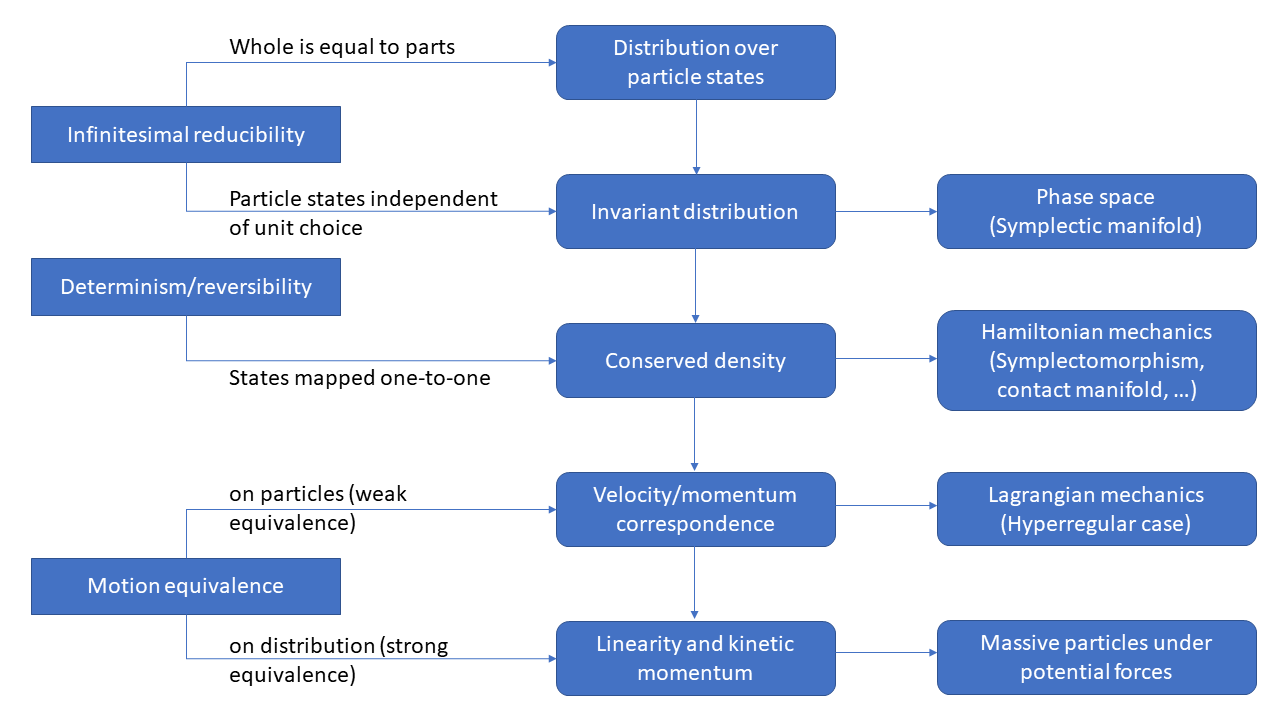
\includegraphics[width=\textwidth]{Diagram.png}
\caption{Physical conditions and corresponding properties and formalisms}
\label{diagram}
\end{figure}

First, a system is \textit{infinitesimally reducible} provided that the state of the whole system is equivalent to specifying the states of its parts (and vice versa). Infinitesimal reducibility distinguishes classical from quantum systems, where the latter are irreducible (we cannot specify the whole state by specifying the states of its subsystems). In the widest sense, a classical system is any infinitesimally reducible system. Colloquially, we can say that the whole state equals the sum of its parts, where we take these infinitesimal parts to be classical particles. 

If a system is infinitesimally reducible, then we can define a distribution $\rho$ over particle states. Furthermore, since particle states are independent of a choice of units, this distribution must be invariant. We show in Section~\ref{infinitesimal} that defining this invariant distribution requires a symplectic manifold, which serves as the phase space of classical mechanics. The physical significance of this symplectic manifold is thereby its connection with the physical condition of infinitesimal reducibility. 
% % I think I could spend more time clarifying reducibility, infinitesimal. Maybe define separately first?

Secondly, a system has \textit{deterministic and reversible evolution} provided that the present state of the system uniquely determines both its future and past states. This condition entails that the invariant distribution $\rho$ is in fact a conserved phase space density. We will show that a classical system which satisfies this condition is Hamiltonian: its phase space is a symplectic manifold that evolves according to Hamiltonian evolution  (i.e. according to a symplectomorphism). We thereby characterize Hamiltonian mechanics as the mathematical framework for infinitesimally reducible systems with deterministic and reversible evolution. Section~\ref{deterministic} justifies this correspondence. 

Finally, some classical systems satisfy a further condition, which we call \textit{motion equivalence}. Motion equivalence holds when the system's trajectory in physical space determines---and is determined by---its evolution in phase space. In other words, knowledge of the trajectory in physical space (e.g. Euclidean three-space $\mathbb{R}^3$) suffices for knowledge of the trajectory in phase space, and vice versa. Physically, knowledge of the trajectory in physical space corresponds to knowledge of position and velocity, while knowledge of the trajectory in phase space requires knowing the system's momentum. Hence, motion equivalence entails a correspondence between velocity and momentum, which formally leads to the framework of Lagrangian mechanics in the hyper-regular domain (Section~\ref{motion}). As a result, Lagrangian mechanics requires that a further physical condition is satisfied, and hence it is less general than Hamiltonian mechanics. 
% % Would be ideal if we can provide some literature support for this notion of motion equivalence. E.g. connecting it with a discussion in Marsden and Abraham foundations of mechanics.

We cannot always determine the evolution of a system in phase space from its trajectory in physical space, since some systems fail to satisfy the condition of motion equivalence. In general, knowing a system's position and velocity does not suffice for knowing its momentum. Considering a photon as a classical particle, we cannot determine its momentum from its trajectory through space.\footnote{Since photons travel at constant speed, we can only recover the direction of momentum from the trajectory, but not the magnitude. Two photons with different momenta can follow the same trajectory.} Hence, knowledge of the physical trajectory of a photon is insufficient for knowledge of its phase space evolution. Different Lagrangians---differing even by more than a constant---can correspond to the same particle trajectories while not agreeing on the total energy, even up to a constant.\footnote{\textcites[1185--1186]{Barrett2} discusses this in the context of the failure of equivalence between the vector field formulations of Lagrangian and Hamiltonian mechanics. In contrast, the trajectories in phase space (encoded by the Hamiltonian vector field) uniquely define the Hamiltonian up to a constant.} Hence, the set of classical systems that satisfy motion equivalence is a proper subset of the classical systems that satisfy the conditions for Hamiltonian mechanics. For at least this reason, Hamiltonian mechanics is more fundamental than Lagrangian mechanics.
% [To do: verify that the scenario of two different Lagrangians---giving rise to the same trajectories in physical space with different energies---arises ONLY when the motion equivalence condition fails. See Curiel 2014, page 42 for his take on this kind of scenario.]

Of course, different definitions of ``Hamiltonian" and ``Lagrangian systems" can result in different interpretive relationships. On our account, Hamiltonian systems are infinitesimally reducible and follow deterministic and reversible evolution.\footnote{Although not sufficient for a definition, Newtonian systems satisfy the motion equivalence assumption. Since Lagrangian systems satisfy all three conditions (infinitesimal reducibility, deterministic/reversible evolution, and motion equivalence), they constitute the intersection of Newtonian and Hamiltonian systems.} We thereby set aside well-known cases of non-deterministic classical systems.\footnote{For discussion of non-deterministic classical systems, see \textcites*[3-4]{Baez}{Earman}{Norton}.} Additionally, we set aside dissipative systems, i.e. those that fail to conserve energy. Possessing a deterministic and reversible evolution is equivalent to being non-dissipative. Our derivation of Lagrangian mechanics in Section~\ref{motion} takes place within the context of conservative systems, so we do not consider systems that satisfy inhomogenous Euler--Lagrange equations. Although both the Lagrangian and Hamiltonian formulations apply to dissipative systems \parencites[\S 10.4]{Cline}, we exclude these.\footnote{Curiel \parencites*[311]{Curiel} acknowledges that the Hamiltonian framework can be extended to treat dissipative systems, although he seems to view it as a virtue of the Lagrangian formulation that it handles dissipative systems with fewer modifications. For details of the Lagrangian approach to dissipative systems, see \textcites[]{Smith}.} Hence, our claim about the fundamentality of Hamiltonian mechanics is restricted to the non-dissipative regime. We will view non-dissipative systems as neither Lagrangian nor Hamiltonian. Finally, our treatment is not restricted to $n$-particle mechanics but applies as well to continuum mechanics (including rigid bodies and fluid mechanics).\footnote{For discussion of continuum mechanics in the context of classical mechanics, see \textcites[]{Wilson}.} Before presenting the derivational details of our argument in Section~\ref{derivation}, we clarify what we mean by ``fundamental."
% For fluid systems, the deterministic/reversible evolution condition applies to the whole system but not for the individual particles due to interactions between these.}
% % Why don't interactions between particles also arise for $n$-particle mechanics? e.g. Newtonian gravity?

% % XXX: try to find a different citation for the claim that dissipative forces can be incorporated in both Hamiltonian and Lagrangian mechanics. Cline libre text might not look the best!

% https://phys.libretexts.org/Bookshelves/Classical_Mechanics/Book%3A_Variational_Principles_in_Classical_Mechanics_(Cline)/10%3A_Nonconservative_Systems/10.04%3A_Rayleighs_Dissipation_Function

%To avoid verbal disputes, it is essential to clarify what falls within the scope of ``classical systems." One way to delimit classical systems is to specify a set of equations that they satisfy---such as Hamilton's equations or the Euler--Lagrange equations. We will instead follow a different approach by delimiting classical systems based on the physical conditions that they satisfy. 





%Figure~\ref{diagram} summarizes our characterization of Hamiltonian and Lagrangian mechanics, in terms of physical conditions and corresponding mathematical structures. Section~\ref{derivation} justifies the logical connection between these physical conditions and corresponding mathematics. Before delving into this derivation, Section~\ref{fundamentality} discusses its philosophical significance.

% One way to motivate the motion equivalence condition: in general, the same trajectory in physical space can correspond to different trajectories in phase space: knowledge of the position and velocity is not sufficient for knowledge of the momentum (e.g. if you do not know the mass of the system). Formally, different Lagrangians can have the same Lagrangian vector field but give rise to Hamiltonians with different Hamiltonian vector fields, as Barrett notes \parencites*[1186]{Barrett2}. In contrast, if two Hamiltonian systems agree on the Hamiltonian vector field, then they must agree on the Hamiltonian, up to an arbitrary constant (whereas two Lagrangian systems can have the same Lagrangian vector field but not agree on the Lagrangian or total energy, even up to a constant)).

% %Overall summary: A classical system is an infinitesimally reducible system. The state space of these systems can be modeled by a symplectic manifold (the physical assumption of infinitesimal reducibility corresponds to the mathematical structure of symplectic manifolds). Classical Hamiltonian systems satisfy the additional conditions of having deterministic and reversible evolutions. These two physical assumptions entail the existence of a symplectic morphism on the state space manifold, making it a contact manifold. Classical Lagrangian systems satisfy a further assumption: keeping track of the trajectories in physical space is equivalent to tracking the evolution of states in phase space. 


\section{Fundamentality, \textit{sans} metaphysics}
\label{fundamentality}

% % done; slip in a citation to Dorr/Hawthorne 2014, to note the independent metaphysical challenges that the notion of naturalness faces, and likewise for a metaphysical notion of fundamentality.

% North argues that ``the structure of physics is the (minimal) structure that is assumed among dynamically equivalent---in classical mechanics: canonically transformed---formulations of a theory. Structure comprises those quantities that remain intact when we transform one allowable coordinatization of the laws into another" [78]

% North's epistemic method for figuring out the structure: ``look at what is invariant under allowable transformations"; this tells us what the structure is [73].

As indicated at the start of Section~\ref{privileging}, we use ``fundamentality" in a non-metaphysical fashion. On our usage, differences in fundamentality amount to differences in generality.\footnote{We also embrace other non-metaphysical uses of ``fundamental," tracking differences in epistemic or conceptual primacy. For instance, we can think of the canonical position and momentum observables as ``epistemically fundamental" because they suffice to completely specify a classical state, fixing its values for all other observables. \textcites[31, 200]{Ruetsche} refers to this as ``fundamental in the physicist's sense." Section~\ref{fundamental} discusses further senses in which the Hamiltonian formalism is more fundamental than Lagrangian mechanics.} Our notion of fundamentality leads to a correspondingly non-metaphysical notion of ``structure." Hamiltonian mechanics employs less structure than Lagrangian mechanics because the former requires fewer physical conditions. Compared with North's \parencites*[]{North} account of structure, our definition has two advantages. First, it avoids metaphysical disputes surrounding perfectly natural or joint-carving properties, which empiricists and pragmatists decry. Secondly, it avoids a technical objection that Swanson and Halvorson \parencites*[]{Swanson} levy against North's more precise mathematical criterion for comparing structure. 

Despite our different commitments, our approach has methodological parallels to North's. We agree with North that it is fruitful to identify both invariants and ``the mathematical structure needed to formulate the theory in an invariant, frame-independent way" \parencites*[65]{North}. Additionally, we agree that it is worthwhile to identify what particular mathematical structure is required by a formulation \parencites[78]{North}. Indeed, we undertake precisely this sort of investigation in Section~\ref{derivation}.\footnote{Curiel also aims to identify the necessary and sufficient mathematical structures for formulating classical mechanics. He sets out to establish the ``geometrical structure necessary (and manifestly sufficient) for the formulation of the Euler--Lagrange equation'' relevant for all kinematically-possible solutions \parencites*[292]{Curiel}. See Section~\ref{Curiel} for discussion.} However, North advocates a metaphysical account of structure, about which we remain agnostic. According to North, ``structure comprises the objective, fundamental, intrinsic features, the ones that remain the same regardless of arbitrary or conventional choices and description" \parencites*[66]{North}. These notions of fundamentality and intrinsicality correspond to differences in joint-carving, where more fundamental or intrinsic features are more joint-carving (or in Lewis's \parencites*[]{Lewis1983} terminology, more natural). 

Owing to our epistemic inabilities to access these putative joints, we do not endorse these metaphysical dimensions of structure or fundamentality.\footnote{For a detailed discussion of difficulties facing the notion of metaphysical naturalness, see \textcites[]{Dorr_Hawthorne}.} While we will argue that Hamiltonian mechanics is significant partly because it elucidates invariant distributions (Section~\ref{density}), this does not entail that additional mathematical structure is physically insignificant or surplus structure. Additional structure may correspond to an additional physically-significant assumption that applies to the system under consideration. Precisely this scenario occurs in the context of Lagrangian mechanics, which requires the additional condition of motion equivalence to hold. Whereas North views Lagrangian mechanics as containing ``excess, superfluous structure" \parencites*[75]{North}, we take this additional condition as optional but still physically significant. Thus, while it is illuminating to identify the minimum mathematical structures necessary for a formulation, additional structure is not automatically rendered physically insignificant. %It corresponds to the physical assumption of motion equivalence, which applies to many classical systems. 
%This characterizes the relationship between Hamiltonian and Lagrangian formalizations of a classical system. 
% classical mechanics also deploys physically significant representations that are not intrinsic to mechanical systems [to do: mention some examples, e.g. in a footnote. The Lagrangian? Cartesian coordinates?]. 

% Emphasize contrast: whereas North is arguing that we should believe that the state space of Hamiltonian mechanics corresponds to that of a classical world (using Occam's razor; inference to the best explanation), we are not trying to figure out which state space structure to believe in more. 
% As Swanson and Halvorson put it, North's argument presupposes ``that statespace structure actually corresponds to some kind of real, physical structure. Many physicists and philosophers of science view statespace as a formal tool for efficiently encoding certain modal commitments of scientific theories, and aid for making calculations and predictions, but not part of the theory's ontology. North's position presupposes some form of statespace realism" [1]. North assuming that there is a fact of the matter regarding the state space of the world.

Additionally, whereas North \parencites*[76]{North} seeks to determine the ``real" fundamental state space structure of the theory---and correspondingly, of a classical world---we remain neutral on this underlying metaphysical question.\footnote{Indeed, Swanson and Halvorson \parencites*[]{Swanson} note that many physicists and philosophers would not interpret statespace structure as part of the theory's ontology, but as a formal device for encoding physical information or as a calculational tool.} Whether Hamiltonian phase space structure is metaphysically fundamental (in a classical world) does not matter for the questions we seek to answer. Regardless of its metaphysical status, Hamiltonian mechanics is physically more fundamental, and we will argue for its epistemic and conceptual primacy as well. Indeed, our argument does not privilege any one of the various mathematical formalizations of Hamiltonian mechanics.\footnote{These include formulating Hamiltonian mechanics on a $2n+1$-dimensional contact manifold, on an extended phase space, on a Poisson manifold, and the standard formulation on a symplectic manifold that we typically use below.} Each of these frameworks has different pragmatic costs and benefits. Hence, it is plausible that there may be no single, uniquely necessary mathematical structure for mechanics, but rather a family of related structures. In other words, there may be no canonical minimal structure for formalizing the relevant physical models and physical assumptions.\footnote{Tulczyjew's reformulation of Hamiltonian mechanics supplies a further reason for viewing symplectic geometry---and hence Hamiltonian mechanics---as conceptually fundamental. According to Teh and Tsementzis, this reformulation shows that  ``the very concept of a classical mechanical system (and not merely the phase space of that system) should be described in terms of symplectic geometry" \parencites*[46]{Teh}.}  Additionally, each of these formalisms references some ``unphysical" coordinates or representational means, whose physical significance is borne out by their fruitfulness in modeling. We return to the physical significance of certain coordinate choices in Section~\ref{fundamental}.
%The mathematical structure that you ``need" might not be unique. Neither one of these three formalizations of Hamiltonian mechanics is necessarily more ``fundamental" or joint-carving than the others. Nevertheless, there are compelling physical and pragmatic motivations for preferring the extended phase space formulation of Hamiltonian mechanics. In this formulation, we gain an invariant Hamiltonian that is the conjugate variable of the proper time, while the normal Hamiltonian (which is not coordinate-invariant) still plays the role of generating time-translations.

North also introduces a technical notion of comparative structure, based on the symmetry group of statespace. According to this criterion, statespace A has more structure than statespace B if the symmetry group of A is a proper subgroup of B's symmetry group \parencites[87-88]{North}.\footnote{This criterion follows from the most charitable reconstruction of North's argument, given by \textcites[]{Swanson}. North sometimes speaks in terms of comparing the dimensions of symmetry groups, which they note leads to counterexamples.} A symmetry group that is a proper subgroup entails that strictly fewer transformations preserve the space's structure. This indicates that statespace A has more mathematical structure to be preserved. These symmetry groups are defined in terms of the coordinate transformations that preserve the space's geometric structure, amounting to re-coordinatizations (redescriptions) of that structure. For Lagrangian systems, North takes the relevant symmetry group to be that of the point transformations, and for Hamiltonian systems, she assumes that canonical transformations play this role. Since point transformations are a proper subgroup of canonical transformations, North's criterion entails that the statespace of Lagrangian mechanics has more structure than the statespace of Hamiltonian mechanics---in virtue of the former having a smaller symmetry group. 

However, Swanson and Halvorson \parencites*[]{Swanson} develop a series of problems for North's argument. Most compellingly, they argue that we cannot in general assume that point transformations and canonical transformations are the proper symmetry groups for Lagrangian and Hamiltonian mechanics, respectively. As they note, Galilean boosts are often symmetry transformations of Lagrangian systems (in the sense of preserving the equations of motion), but they are not point transformations. Additionally, the two-body problem admits canonical transformations that map physically distinct solutions to each other (specifically, solutions whose orbits possess the same energy but different eccentricity).\footnote{For more details on the classical two-body problem, see \textcites[]{Belot}.} Hence, we cannot straightforwardly compare the structure of Lagrangian and Hamiltonian mechanics in terms of the symmetry groups of their statespaces. 

Advantageously, our criterion for comparing Hamiltonian and Lagrangian mechanics avoids the criticisms that Swanson and Halvorson develop against North. Hamiltonian mechanics has less structure than Lagrangian mechanics simply in the sense of logical strength: a system must satisfy strictly fewer physical conditions in order to be Hamiltonian. Whereas to be Lagrangian, the system must also satisfy the assumption of motion equivalence. The assumption of motion equivalence places an additional constraint on the Hamiltonian, a constraint that need not be satisfied in general. 

%% Not sure if it is worth raising the following worry. If so, need to fix/clarify the response, which is sketchy.
%Nevertheless, based on the equivalence between the tangent bundle and cotangent bundle formulations of Lagrangian and Hamiltonian mechanics, one might wonder whether there could be a ``correspondingly general formulation of Lagrangian mechanics" that is analogous to the symplectic but-not-cotangent-bundle formulation of Hamiltonian mechanics \parencites[1182]{Barrett2}. For, if there were, then this formulation of Lagrangian mechanics might be more general than the cotangent bundle formulation of Hamiltonian mechanics. And thus, there would be an analogous sense in which Lagrangian mechanics is more fundamental than Hamiltonian mechanics, undercutting our argument. Fortunately, it is implausible that there could be a suitable generalization of Lagrangian mechanics. In going from the cotangent bundle formulation of Hamiltonian mechanics to the symplectic manifold formulation, we lose some globally-defined structure. This is analogous to moving from the space of globally-Euclidean manifolds to the space of locally-Euclidean manifolds. Yet, it is not clear how Lagrangian mechanics could remain well-defined while throwing away global structure from the tangent bundle. For the action seems to be inherently a globally-defined quantity, as an integral defined over a trajectory.


% Plausibly, move the following directly after our claim that our notion of fundamentality/structure comparison avoids the objections of Swanson/Halvorson against North's:



% Way to motivate that the motion equivalence assumption further constrains the Hamiltonian: the Hamiltonian already defines a relationship between conjugate momentum and velocity (through ($dq/dt = \partial H / \partial p$) ). Motion equivalence provides a further constraint on this relationship, and hence a further constraint on the Hamiltonian. 

% As defined, our notions of fundamentality and structure are not metaphysical in nature.

%Finally, our argument does not privilege any one of the at least three different mathematical ways of formalizing Hamiltonian mechanics [mention these three formalisms and provide references]. Each of these frameworks has different pragmatic costs and benefits. Hence, unlike North, we are comfortable acknowledging that the mathematical structure that you ``need" might not be unique. There might not be a single canonical minimal structure for formalizing the relevant physical models and physical assumptions. Neither one of these three formalizations of Hamiltonian mechanics is necessarily more ``fundamental" or joint-carving than the others. And in some sense, each of these formalisms references some ``unphysical" coordinates or representational means. Nevertheless, there are compelling physical and pragmatic motivations for preferring the extended phase space formulation of Hamiltonian mechanics. In this formulation, we gain an invariant Hamiltonian that is the conjugate variable of the proper time, while the normal Hamiltonian (which is not coordinate-invariant) still plays the role of generating time-translations.
% One con of this extended phase space formulation: the Hamiltonian constraint is both a constraint and the generator of time evolution; hence, it must be defined in the neighborhood of the actual states, so the values it provides outside of these neighborhoods should be unphysical, yet they encode the equations of motion.
% Should we remark on the claim that the only structure we need is whatever is sufficient to define densities locally? Hence, we need just the symplectic form but not the cotangent bundle?
% E.g. in the extended phase space formulation, the equations of motion come from derivatives of the Hamiltonian constraint over the variables, but this constraint is defined on unphysical points. These unphysical points are plausibly a mathematical artifact, although they supply a nice tool/method for understanding physically significant aspects of the representation.

% One way to motivate the motion equivalence condition: in general, the same trajectory in physical space can correspond to different trajectories in phase space: knowledge of the position and velocity is not sufficient for knowledge of the momentum (e.g. if you do not know the mass of the system). Formally, different Lagrangians can have the same Lagrangian vector field but give rise to Hamiltonians with different Hamiltonian vector fields, as Barrett notes \parencites*[1186]{Barrett2}. In contrast, if two Hamiltonian systems agree on the Hamiltonian vector field, then they must agree on the Hamiltonian, up to an arbitrary constant (whereas two Lagrangian systems can have the same Lagrangian vector field but not agree on the Lagrangian or total energy, even up to a constant)).

% Claim to think about: GC was arguing on 10-12 that you could handle classical systems in the Hamiltonian framework with just a differential manifold and no symplectic structure. This would contradict North's indispensability claim that Hamiltonian symplectic structure is necessary for treating classical systems. E.g., North footnote 31: ``The symplectic form is crucial to determining the motion, since the same Hamiltonian can induce different flows for different symplectic forms" [76]. North takes this as an argument for why we cannot eliminate the symplectic form in an attempt to get at even less structure. We need it to define the dynamics.



\section{Deriving Hamiltonian and Lagrangian mechanics}
\label{derivation}

% [To do: figure out how to flag to the reader that they can skip/skim some parts of this derivation section without loss of understanding for later sections]. E.g., `Readers who are more interested in the significance of invariant phase space densities or the geometric action principle can feel at peace skipping ahead.' But, presumably, part of the stuff on invariant densities is relevant for Section~\ref{density}? Figure out how to finesse this

This section justifies the physical and mathematical relationships in Figure~\ref{diagram}.
Sections~\ref{infinitesimal}-\ref{deterministic} derive the formalism of Hamiltonian mechanics from the assumptions of infinitesimal reducibility and deterministic/reversible evolution. Section~\ref{motion} shows how systems that satisfy the further condition of motion equivalence can be treated within the formalism of Lagrangian mechanics. We thus demonstrate in detail our methodology of deriving  relevant mathematical structures from underlying physical conditions.

% Is it worth emphasizing/highlighting any particularly important parts of the derivation up front? 

\subsection{Infinitesimal reducibility}
\label{infinitesimal}

First, we will show that a classical phase space arises if a system satisfies the following physical condition:

\begin{quotation}
\noindent
\textit{Infinitesimal reducibility}: the state of the system is reducible to the state of its infinitesimal parts. That is, giving the state of the whole system is equivalent to giving the state of its parts, which is equivalent to giving the states of those parts, and so on.
\end{quotation}

\noindent
This assumption characterizes classical systems as those whose infinitesimal parts completely specify the state of the system. We define a \textit{classical particle} as one of these infinitesimal parts, namely the limit of recursive subdivision.\footnote{For discussion of the status of extensionless point particles within classical mechanics, see \textcites[]{Butterfieldpoints}.}
%comment on how this characterization of infinitesimal particles relates to standard philosophy of physics interpretive disputes over the status of point particles in classical mechanics. Butterfield characterizes particles as extensionless.

Let $\mathcal{C}$ be the state space for the whole system, so that any point $c \in \mathcal{C}$ represents a particular state of the whole system. Given infinitesimal reducibility, a classical system consists of a collection of classical particles. Let $\mathcal{S}$ be the state space for the particles, so that each point in $\mathcal{S}$ describes a possible state of a classical particle. Then for each state $c \in \mathcal{C}$ there exists a unique distribution $\rho_c : \mathcal{S} \to \mathbb{R} $ that describes the state of $c$'s parts. That is, the state of the whole system is a distribution over its infinitesimal parts. This distribution describes the proportion of classical particles in any particular state.

If $\mathcal{S}$ is a discrete space, we define [XXX: $\rho_c$ should have lowercase 'c' consistently] $\mu(U) = \sum\limits_{s \in U} \rho_c(s)$ so that $\mu(\mathcal{S})$ gives us the size of the system and $\mu(U)/\mu(\mathcal{S})$ gives us the fraction of the particles that can be found in the region $U$. That is all.\footnote{The discrete is also far less interesting because discrete quantities cannot change continuously over time, meaning that they must be constant. For details see \textcites[]{AoPPhy1} [omit this for review; or find alternative source].}
%[is region U in the state space C or S. I assume in S.].
% % XXX could try to find justification/derivation for the state space being a manifold in the Kevin Kelly book, or could cite the math paper with Greenfield; proposition 6.2. Try to include a better gloss/motivation for this claim (basic idea: if time is continuous, trajectories in state space must be continuous, local structure must be compatible). Curiel paper might also have a brief justification/motivation, if I recall

In the continuous case, when $\mathcal{S}$ is a manifold, the story is more complicated. Let us call \textit{state variables} a set of quantities $\xi^a$ that fully identify a state so that $\xi^a: \mathcal{S} \to \mathbb{R}^n$ is an invertible function between each state and the numeric values of the variables.\footnote{In the language of manifolds, these $\xi^a$ are called `coordinates'. However, we will have multiple manifolds and, to avoid confusion, we will specifically call state variable the coordinates of the state space. [XXX: would remove, terminology that we adopt when speaking about coordinate transformations, coordinate invariance, and coordinate independence.]} The goal is to define $\mu(U) = \int_U \rho_c(s) d\mathcal{S} = \int_U \rho_c(\xi^a) d\xi^a$ and the issue is that we need to make sure that the equation makes dimensional sense: we need to make the units work.

On one side, $\rho_c : \mathcal{S} \to \mathbb{R}$ is only a function of the state, and therefore its value is independent of the choice of units for the state variables: it is a scalar function and, as all scalar functions, it is coordinate independent. However, we must be able to express $\rho_c : \mathbb{R}^n \to \mathbb{R}$ as a function of the state variables, and when we do so its integral $\int_U \rho_c(\xi^a) d\xi^a$ must also be invariant under change of state variables: $\rho_c$ has to transform like a density. Densities are not invariant: they transform with the Jacobian. For $\rho_c$ to remain unchanged, the Jacobian determinant must in fact equal one and it must be a pure number. In other words, while we need to be able to change the units used by the state variables $\xi^a$ to identify the particle states, the units for $\rho_c$ must remain the same so that the density does not change its numeric value.\footnote{Formally, we can express this argument as a chain of equalities: $\rho_c(\hat{\xi}^b)=\rho_c(s(\hat{\xi}^b))=\rho_c(s(\xi^a))=\rho_c(\xi^a) = \left|\frac{\partial \hat{\xi}^b}{\partial \xi^a} \right| \rho_c(\hat\xi^b)$, where $\rho_c(\xi^a)$ and $\rho_c(\hat{\xi}^b)$ represent the same distribution as expressed over different state variables and $s(\xi^a)$ and $s(\hat{\xi}^b)$ represent the same particle state as expressed by the different variables. Note that $\rho_c(s(\hat{\xi}^b))$ shows how the distribution depends on the state variables only through the particle state.} We will now show that in order for the distribution to satisfy these two constraints, the classical phase space must be at least a symplectic manifold. In other words, having symplectic manifold structure is a necessary condition for the distribution over particle states to transform as a density and a scalar function.

Let us define a \textit{unit variable} $q \in \xi^a$ as a particular state variable that defines a unit. For instance, $q$ might be position, defined in units of meters. Two unit variables are \textit{independent} if one unit variable can be changed without changing the other. For example, one can measure the vertical position in meters while measuring the horizontal position in miles.  In general, the unit variables $q^i$ are the subset of the state variables that define the unit system, which is needed to relate the properties of the system to the measured values. The idea is that the $q^i$ not only determine the units for themselves, but for all other state variables. A \textit{change of units} is therefore a map $\hat{q}^j = \hat{q}^j(q^i)$ that defines new unit variables in terms of the old unit variables alone. Since the unit variables define the units for all state variables, this change must induce a unique change of state variables $\hat{\xi}^b = \hat{\xi}^b(\xi^a)$ for all variables.
% [XXX: coordinates -> unit variables]

% % Ask GC if instances of `state variables' in the next paragraph are correct; i.e. `state variables' rather than `coordinates'
% On physical grounds, [XXX: I'd say it's more mathematical grounds] 

%This is because the distribution is a function only of the states, rather than of the particular choice of coordinates. 
 % Classical phase space (i.e. a symplectic manifold) is the only space that satisfies these constraints on the distribution. 
%(in manifold terminology, these are known as coordinates)

Let us consider the simplest case: suppose that a single unit variable $q $ suffices to define the unit system for the particle state space. Then, the state variables are given by a set $\xi^a = \{ q, k^\alpha \}$, where \textit{prima facie} the index $\alpha$ could be any non-negative integer. We will show that, in fact, there must be exactly one $k^i$ variable, conjugate to the single $q$ variable. 
% We further assume that $q$ fully defines the units for all state variables. [Is there a way to physically motivate this assumption, beyond this being a constitutive role of the position-like state variables?]

As we said, the units of the particle density $\rho_c$ should not be affected by a change of units of the state variables. So suppose we change the units by transforming $q$ to a new unit variable $\hat{q}=\hat{q}(q)$. Call the new state variables $\hat{\xi}^b = \{ \hat{q}, \hat{k}^\beta\}$. As shown above, the Jacobian determinant $\left|\frac{\partial \hat{\xi}^b}{\partial \xi^a} \right|$ must equal one. Assume for contradiction that there is only one state variable, so that there are no $k^i$ variables. Then we would have $\left|\frac{\partial \hat{\xi}^b}{\partial \xi^a} \right| = \left|\frac{\partial \hat q}{\partial q} \right| = 1$. But this would mean the unit change cannot be arbitrary. Therefore we must have two or more state variables, requiring at least one $k^\alpha$ variable. 

\begin{comment}
%Longer justification for the Jacobian determinant equaling one. 

 As defined, $\rho_c$ is a function from the particle state space $\mathcal{S}$ to the reals. We can define $\rho_c$ on the units by taking advantage of an invertible function $s: \mathbb{R}^n \to \mathcal{S}$ mapping a particular value of the units $\hat{\xi}^b$ to a point in the particle phase space $\mathcal{S}$. Hence, by definition $\rho_c(\hat{\xi}^b):= \rho_c(s(\hat{\xi}^b))$. [Is this function $s$ the inverse of the coordinate mapping $\xi^b$?]. Then, since the physical state is independent of the coordinates, the state $s(\hat{\xi}^b)$ is the same state as $s(\xi^a) $ defined in terms of the original units $\xi^a$. Again, by definition, $\rho_c(s(\xi^a))=\rho_c(\xi^a) $. Since the distribution transforms as a density, it follows that $\rho_c(\xi^a)$ must equal the product of the Jacobian determinant $\left|\frac{\partial \hat{\xi}^b}{\partial \xi^a} \right| $ times the density defined over the transformed units: $\rho_c(\xi^a) = \left|\frac{\partial \hat{\xi}^b}{\partial \xi^a} \right| \rho_c(\hat\xi^b)$. We can summarize the argument so far as a chain of equalities:

\begin{equation*}
\rho_c(\hat{\xi}^b)=\rho_c(s(\hat{\xi}^b))=\rho_c(s(\xi^a))=\rho_c(\xi^a) = \left|\frac{\partial \hat{\xi}^b}{\partial \xi^a} \right| \rho_c(\hat\xi^b)
\end{equation*}

\noindent
Therefore the Jacobian $\left|\frac{\partial \hat{\xi}^b}{\partial \xi^a} \right|$ must equal one. 

\end{comment}




Next, we show that in fact there must be exactly one $k$ variable, conjugate to the single $q$ variable. Using the fact that the Jacobian determinant equals one, we determine how the state variables $k^\alpha$ must change in order to compensate the change from $q$ to $\hat q$. Since $\hat{q}$ depends only on $q$, $\frac{\partial \hat{q}}{\partial k^\alpha} = 0$. Hence, the Jacobian is a lower triangular block matrix: 



\begin{equation}
%\begin{aligned}
|J| = \left|\frac{\partial \hat{\xi}^b}{\partial \xi^a} \right| = \begin{vmatrix}
\frac{\partial \hat{q}}{\partial q} & \frac{\partial \hat{q}}{\partial k^\alpha} \\
\frac{\partial \hat{k}^\beta}{\partial q} & \frac{\partial \hat{k}^\beta}{\partial  k^\alpha} 
\end{vmatrix} = \begin{vmatrix}
\frac{\partial \hat{q}}{\partial q} & 0 \\
\frac{\partial \hat{k}^\beta}{\partial q} & \frac{\partial \hat{k}^\beta}{\partial  k^\alpha}
\end{vmatrix}
%\end{aligned}
\end{equation}

\noindent
The determinant of a triangular block matrix equals the product of determinants of the block matrices along the diagonal: $ \left|\frac{\partial \hat{\xi}^b}{\partial \xi^a} \right| =  \left|\frac{\partial \hat{q}}{\partial q}\right| \left|\frac{\partial \hat{k}^\beta}{\partial k^\alpha}\right|$. For the Jacobian determinant to equal one, we must therefore have  $\left|\frac{\partial \hat{k}^b}{\partial k^a} \right| =   \left|\frac{\partial \hat{q}}{\partial q}\right|^{-1}$. Since $\hat q$ is a function only of $q$, $\frac{\partial \hat{q}}{\partial q}$ is a total derivative, so we obtain the inverse by swapping the numerator and denominator. Hence, we see that $\left|\frac{\partial \hat{k}^\beta}{\partial k^\alpha} \right| = \left|\frac{\partial q}{\partial \hat q} \right|$. 
%  $\left|\frac{\partial \hat{q}}{\partial q}\right|^{-1} = \left|\frac{\partial q}{\partial \hat q} \right|$. 

This equation provides only a single constraint, placed on the determinant of the transformation from $k^\alpha$ to $\hat{k}^\beta$. Hence, if there were three or more $\xi^a$ variables, this constraint would be insufficient to recover the transformation of the $k^\alpha$ uniquely. Yet in this case, $\hat q$  would not fully define the units for all other state variables, contrary to assumption. Consequently, there must be exactly two state variables: $q$ and a single $k$. So in the case of a single $q$ variable, defining a coordinate-independent density requires a two-dimensional manifold.

\begin{comment}
\begin{equation}
\left|\frac{\partial \hat{q}}{\partial q}\right| \left|\frac{\partial \hat{k}^b}{\partial k^a}\right| - \left|0\right| \left|\frac{\partial \hat{k}^b}{\partial q}\right|
= \left|\frac{\partial \hat{q}}{\partial q}\right| \left|\frac{\partial \hat{k}^b}{\partial k^a}\right|.
\end{equation}
 so $\left|\frac{\partial \hat{\xi}^b}{\partial \xi^a} \right| = \left|\frac{\partial \hat q}{\partial q} \right|\left|\frac{\partial \hat{k}^b}{\partial k^a} \right|$: 
\end{comment}

Extending to the general case, recall that two unit-variables are independent if changing the units for one does not change the units for the other. Suppose our particle state space $\mathcal{S}$ is such that its units are fully defined by $n$ independent unit-variables $q^i$. If we change the first unit-variable $q^1$ without changing the others, then the variable $k_1$ must change as before, so that the density remains invariant. Likewise, transforming the second unit-variable $q^2$ in the same way (while fixing $k_1$) requires a corresponding $k_2$. In the end, we will find that $\mathcal{S}$ is $2n$-dimensional, and the state variables are $\xi^a = \{ q^i, k_i \}$. We define an \textit{independent degree of freedom} as the space charted by a pair of such variables.

We can now show that $\mathcal{S}$ must have at least the structure of a symplectic manifold. Defining an invariant density requires the existence of infinitesimal areas. Therefore we need a two-form $\omega$ that assigns an infinitesimal area to each infinitesimal surface. This lets us define integrals of the form $\int_{\Sigma} \rho_c \omega(d\Sigma)$, for $\Sigma \subset \mathcal{S}$ (i.e. the fraction of the system whose parts are in the region $\Sigma$ of state space $\mathcal{S}$). Because degrees of freedom are---at least locally---independent, the total number of states in a volume is the product of the possible configurations of each degree of freedom. This means the volume form is given by $\omega^n$. Importantly, the volume form cannot be degenerate because otherwise there would be a `volume' in state space that could not contain states. But such a region of state space would---by definition---not be a volume. Therefore the form $\omega$ itself cannot be degenerate (for otherwise, we would have states that are not counted by it). 
% % Invariant densities can only be assigned to infinitesimal areas. Get a citation for this claim

Next, we show that $\omega$ must be closed, using the fact that degrees of freedom are independent. If we translate a surface along an independent degree of freedom, this does not change the area of the surface, meaning that the number of states on that surface is invariant. Consider a parallelepiped, whose opposite sides have equal areas. Taking the integral over this closed surface (over the parallelepiped), opposite sides provide equal and opposite contributions. Hence, the integral over this closed volume must equal zero. This shows that the 2-form $\omega$ must be closed. Therefore $\mathcal{S}$ must come equipped with a two-form $\omega$ that is closed and not degenerate, and therefore $\mathcal{S}$ is a symplectic manifold.

The units we choose for $\omega$ are really the units we choose to count states over an independent degree of freedom, which agrees with the practice in statistical mechanics. The density $\rho_c$, when normalized, is given in terms of the inverse of that unit. In accordance with the standard conventions in quantum mechanics and statistical mechanics, the $k_i$ are given in terms of inverse units of the respective $q^i$, such that $dq^i \wedge dk_i$ is a pure number. We then use $\hbar$ to define the unit for state counting and therefore set $\omega = \hbar dq^i \wedge dk_i = dq^i \wedge dp_i$ where $p_i = \hbar k_i$.
% % the `motivation' section of the wiki page on symplectic manifolds provides a different style of derivation for the 2-form being non-degenerate and closed. 

In terms of physics, then, a set of canonical coordinates is a set of state variable that expresses the density in the correct unit. A canonical transformation is one that preserves the unit and the numerical value of the density. A change of unit is a special type of canonical transformation: one where we have an arbitrary change in the unit variables and an induced (covariant) change in the conjugate variables.

The conclusion is that, under the infinitesimal reducibility assumption, a state $c$ of the system is a coordinate-invariant distribution over the state space $\mathcal{S}$ of its infinitesimal parts. We have shown that the state space of the particles must be a symplectic manifold. Additionally, any symplectic manifold structure supports the definition of coordinate-invariant distributions: any scalar function can be integrated using the symplectic form in a coordinate-invariant way. Therefore the symplectic structure is exactly the structure needed to define an invariant density. Section~\ref{density} describes further interpretive consequences of this connection between invariant densities and symplectic structure.
% % [XXX: clarify/clean-up this ending. also, emphasize/foreshadow the physical signifiance of the distribution and density]. also, clarify relationship b/w distribution (ontology) and density (epistemic access to/representation of this ontology)
%Symplectic manifold structure is exactly the structure needed to define an invariant density. 
% Could connect this with the earlier discussion of North's methodology of seeking coordinate-invariants, from section~\ref{fundamentality}.

%since the degrees of freedom are independent, the number of states on a surface does not change if we translate that state across independent degrees of freedom. If we imagine a parallelepiped, the integral over the surface must be zero (the integrals over opposite sides are equal and opposite) [explain/justify this more clearly. Is this coming from the two-form being antisymmetric?]. 
%
%if degenerate form, would have states that are not counted by the form. 


% Which is the only type of manifold that supports coordinate-invariant distributions

\subsection{Deterministic and reversible evolution}
\label{deterministic}

Next, we focus on those classical systems that are deterministic and reversible. This amounts to satisfying the following joint condition:

\begin{quotation}
\noindent
\textit{Deterministic and reversible evolution}: given the present state of the system, all future (determinism) and past (reversible) states are uniquely identified.

\end{quotation}

In our case, this applies to both the state of the whole system and to the state of its parts. Let $\lambda: \mathbb{R} \to \mathcal{S}$ be the evolution over time of the state of a particle. Assuming deterministic and reversible evolution, the initial state $s_0 = \lambda(t_0)$, at the initial time $t_0$, uniquely identifies the state of the system. Moreover, if $\rho(\lambda(t_0), t_0)$ is the density associated to the initial state at the initial time, we must have that $\rho(\lambda(t), t) = \rho(\lambda(t_0), t_0)$, i.e. the density remains the same throughout the evolution. In other words, all particles that begin in a given initial state must end up in the same final state and vice-versa.  
%[could two different particles occupy the same initial state?].
%[what exactly does `initial particle' mean? Do we mean the initial state of the composite system or just a particular particle?] 

Now consider the integral $\int_{\Sigma} \rho_c \omega(d\Sigma)$. The region $\Sigma$ will be mapped to a new region, but the fraction of the system found in both the old and new regions must be the same. Since both the integral and $\rho_c$ must remain constant during the evolution, the two-form $\omega$ must also remain the same. That is, the areas in phase space must be mapped to areas of equal size, and independent degrees of freedom must be mapped to independent degrees of freedom (otherwise, volumes would not be mapped to equal volumes, which would violate determinism). The evolution is therefore a symplectomorphism and corresponds to Hamiltonian evolution. 

Intuitively, this argument is the inverse of Liouville's theorem: instead of positing Hamiltonian evolution and finding conservation of areas and volumes, deterministic and reversible evolution imposes the conservation of areas and volumes (i.e. sets of states are mapped to sets of states of equal size) which leads to Hamiltonian evolution. In summary, we have shown that any system that satisfies the conditions of both infinitesimal reducibility and deterministic/reversible evolution is a classical Hamiltonian system.


\subsection{Motion equivalence}
\label{motion}

Having recovered classical Hamiltonian mechanics, the laws of evolution are further restricted when the following condition holds:

% [to do: make the footnote regarding connection to Marsden and Abraham more precise. Might want to flag that their theorem is expressed in terms of the Lagrangian vector field and corresponding Hamiltonian vector field (obtained via Legendre transformation) having the same base integral curves. These base integral curves encode how particles evolve over time. Should I also elaborate on how one can interpret motion equivalence in terms of the theories having the same empirical content? This is how Barrett interprets the Marsden and Abraham theorem 3.6.2]
\begin{quotation}
\noindent
\textit{Motion equivalence assumption}: the motion of the system (i.e. trajectories in physical space-time) suffices to recover its dynamics (i.e. evolutions in state space) and vice-versa.\footnote{ \textcites[]{Abraham}, Theorem 3.6.2 shows that in the hyper-regular domain, Lagrangian and Hamiltonian mechanics describe the same evolution of particle positions over time (see \textcites[1180-1181]{Barrett2} for discussion). Motion equivalence can be understood as the converse of this theorem: assuming that Lagrangian and Hamiltonian mechanics agree on particle evolutions, we derive that the Legendre transformation is well-defined in the hyper-regular domain.}
\end{quotation}

If we focus on the parts of the system, this means that for every evolution in phase space there should be one and only one trajectory in physical space. Note that each space variable $x^i$ is a unit variable, i.e. a state variable that defines a unit. In fact, the trajectories can be fully described only by these unit variables. For, to specify a trajectory, we need epistemic access to a unit system, where the number of independent units is determined by the dimensionality of physical space. It follows that (i) $x^i = q^i$, (ii) each $q^i$ is paired with a conjugate $p_i$, and (iii) each state $\{q^i, p_i\}$ corresponds to one and only one trajectory in physical space. At each point $x^i$, then, there must be infinitely many trajectories, one for each possible combination of $\{p_i\}$. Since these trajectories are differentiable in $x^i$, we can define a velocity $v^i = d_t x^i$. If the equations of motion were such that the velocity were a function of only the unit variables (i.e. $v^i=v^i(q^i)$), then motion equivalence would fail. For if both $x^i$ and $v^i$ were a function of only $q^i$, this relationship would not be invertible because of dimensional considerations (a surjective function from an $n$-dimensional manifold to a $2n$-dimensional manifold cannot be invertible). Hence, we must have $v^i=v^i(q^j, p_k)$, so that knowledge of the state in phase space suffices for knowledge of the trajectory. If motion equivalence holds, then this relationship must be invertible, meaning that knowledge of the trajectory suffices for knowledge of the phase space state. For systems that satisfy the motion equivalence condition, then, the following relationships hold at any given time:
\begin{equation}\label{weak_equivalence}
\begin{aligned}
x^i &= q^i \\
v^i &= d_t x^i = v^i(q^j, p_k)
\end{aligned}
\end{equation}

<<<<<<< Updated upstream
In this case---which we call \textit{weak equivalence}---$v^i(q^j, p_k)$ is invertible at every $q^i$. Therefore, for fixed $q$, the Jacobian matrix  $\frac{\partial v^i}{\partial p_j}$ must be invertible. Since $v^i = d_t q^i = \frac{\partial H}{\partial p_i}$, the Hessian $\frac{\partial^2 H}{\partial p_i \partial p_j} = \frac{\partial}{\partial p_i} (\frac{\partial H}{\partial p_j})$ equals the Jacobian $\frac{\partial v^i}{\partial p_j}$. [XXX: Has $H$ been introduced?] Since the Jacobian is invertible, the Hessian must be non-zero everywhere, and therefore it must have the same sign everywhere, which we take to be positive. Weak equivalence allows us to express particle states in terms of either position/momentum or position/velocity variables. These are exactly the cases where a Lagrangian can be constructed, and where the Lagrangian leads to a unique solution (via the stationary action principle). Hence, weak equivalence suffices for the existence of a hyper-regular Lagrangian.\footnote{Weak equivalence corresponds to a general treatment of Lagrangian mechanics that does not presuppose Riemannian geometry. As we discuss in Section~\ref{Curiel}, Equation~\ref{weak_equivalence} corresponds to the kinematical constraints central to Curiel's \parencites*[]{Curiel} argument for privileging Lagrangian mechanics.}

Whereas weak equivalence involves motion equivalence at the level of particle states, \textit{full equivalence} extends this to the entire distribution, i.e. the composite state of the system. Full equivalence holds when we can express the distribution---represented by the density---in terms of position and velocity variables. Formally, this requires that $\rho(q^i, p_j) = |J| \rho(x^i, v^j) = \left|\frac{\partial v^i}{\partial p_j}\right| \rho(x^i, v^j)$ since
\begin{equation}
\begin{aligned}
|J| &= \begin{vmatrix}
\frac{\partial x^i}{\partial q^j} & \frac{\partial x^i}{\partial p_j} \\
\frac{\partial v^i}{\partial q^j} & \frac{\partial v^i}{\partial p_j}
\end{vmatrix}
= \begin{vmatrix}
\delta^i_j & 0 \\
\frac{\partial v^i}{\partial q^j} & \frac{\partial v^i}{\partial p_j}
\end{vmatrix} \\
&= \left|\delta^i_j\right| \left|\frac{\partial v^i}{\partial p_j}\right| 
= \left|\frac{\partial v^i}{\partial p_j}\right|.
\end{aligned}
\end{equation}
Note that while the value given by $\rho(q^i, p_j)$ is invariant under unit changes, the value given by $\rho(x^i, v^j)$ depends on the choice of units through $\left|\frac{\partial v^i}{\partial p_j}\right|$. If $x^i$ truly sets the unit system by itself, then $\left|\frac{\partial v^i}{\partial p_j}\right|$ must be a function of position only, since the position variables---by themselves---define the units. Similar considerations hold for marginal distributions (i.e. distributions on a subset of the unit variables), entailing that all components of $\frac{\partial v^i}{\partial p_j}$ must be a function of position only. We set:\footnote{In Section~\ref{dependence}, we will see that $g^{ij}$ corresponds to the Riemannian metric, since $\partial v^i/\partial p_j$ it is a function only of position.}
\begin{equation}
\begin{aligned}
\frac{\partial v^i}{\partial p_j} = \frac{1}{m} g^{ij} \\
\frac{\partial p_j}{\partial v^i} = m g_{ji}
\end{aligned}
\end{equation}
where $m$ is the unit conversion constant between velocity and conjugate momentum, while $g_{ij}$ represents the linear dependency of the velocity on the momentum. 

If we integrate, we have:
\begin{equation} \label{linear_relationship}
\begin{aligned}
v^i = \frac{1}{m} g^{ij}(p_j - A_j) \\
p_j = m g_{ji} v^i + A_j
\end{aligned}
\end{equation}
where $A_j$ are arbitrary functions. Note that:
\begin{equation}
v^i = d_t q^i = \frac{\partial H }{\partial p_i} = \frac{1}{m} g^{ij}(p_j - A_j) \\
\end{equation}
We integrate yet again and find:
\begin{equation} \label{massive_Hamiltonian}
H = \frac{1}{2m} (p_j - A_j) g^{ij}(p_j - A_j) + V \\
\end{equation}
where V is another arbitrary function. We recognize this as the Hamiltonian for massive particles under potential forces, covering both classical electrodynamics and classical Newtonian gravitation. For example, $A$ can play the role of the magnetic vector potential, with $V$ playing the role of the electric potential. Whereas Curiel \parencites*[]{Curiel} argues that this Hamiltonian requires the imposition of \textit{ad hoc} conditions, we take ourselves to have given an eminently natural construction of it. We return to this point in Section~\ref{Curiel}, using it to defuse Curiel's argument for the primacy of Lagrangian mechanics.

This completes our central argument for privileging Hamiltonian mechanics over Lagrangian mechanics. We have seen that Lagrangian systems are a proper subset of Hamiltonian systems, specifically those Hamiltonian systems that also satisfy the motion equivalence condition. In the remainder of this essay, we provide further reasons for privileging Hamiltonian mechanics. The next section describes how Hamiltonian mechanics provides the natural setting for the invariant density, describing the matter content of the theory [XXX: matter content of the theory seems like an odd phrase]. Section~\ref{fundamental} argues that the invariant phase space density is more fundamental than the state variables, since conjugate momentum is a gauge-dependent quantity. We then turn in Section~\ref{Lagrangian} to provide a geometric interpretation of the principle of stationary action within Hamiltonian mechanics. Our construction makes manifest the gauge redundancy of the Lagrangian, providing a further reason to privilege the Hamiltonian. Finally, we respond to Curiel's arguments against the fundamentality of Hamiltonian mechanics.



\section{The physical significance of invariant densities}
\label{density}

\begin{comment}
* ``Fundamentality" because it makes the physics more prominent. Some people use coordinate-free/independence as necessary conditions for fundemantaly/physical significance. This means coordinates do not appear in the definition. Yet, densities require coordinate for the definition, therefore cannot be coordinate-free/independent, therefore there are some physically significant quantities that do not satisfy that. Why fundamental??? (reverse mathematics? fundamental because it recovers the correct math from the physical assumption?)

---
Section on densities and riemmanian geometry. (Gabriele)

* A paragraph to show how densities work. In general are coordinate dependent and you can't simply compare values at different points. This is the case in Lagrangian mechanics because both differentials in position vary contravariantly.

* Contrast this with densities over position and velocity. But! We can understand some aspects of Riemmanian geometry in terms of how states densities are represented over position and velocity. Hyper-regularity allows us to express densities from "states" to "kinematic variables". The fact that this expression depends only on position (and not on velocity), tells us we have a Riemannnian manifold. Norm of the metric tensor gives us the ``conversion'' factor. Note that norm of the metric tensor in general depends on the coordinate system and is in general point-dependent. There always exists a coordinate system in which the norm of the metric tensor is constant. The conversion factor for marginal distributions is linked to the eigenvalues along each coordinate. Flatness means there exists a coordinate system where we can factorize the distribution (if it factorizes in phase space), which is exactly the Cartesian coordinate system. (Note, we can always factorize in phase space) -> Therefore this focus on densities also allows us to get a better intuition even on the tangent space. [Still need to incorporate much of this discussion]

\end{comment}

Hamiltonian mechanics is more fundamental than Lagrangian mechanics because Hamiltonian systems require fewer physical conditions. While this provides one reason to privilege Hamiltonian mechanics, it is not the only one. In this section, we argue that the special relationship between Hamiltonian mechanics and invariant densities provides a further reason to privilege Hamiltonian mechanics. Additionally, we argue that viewing physics through the lens of invariant densities has much to commend it. In general, it provides a better understanding of classical systems. 

In the Hamiltonian formalism, the density has the following desirable property: we can compare the density point-wise across phase space. If the scalar value of the density at one point is larger than another, this entails that the density is higher at that point of phase space. Physically, this means that there is more matter at this point. Likewise, if the scalar value of the density is the same at two different points, this entails that there is the same amount of stuff at those points. For brevity, we'll refer to this as the property of \textit{point-wise comparison}. Point-wise comparison requires a coordinate-invariant density. As the derivation in Section~\ref{deterministic} shows, to guarantee the existence of an invariant density, we must define state space over a symplectic manifold. In other words, to generically have a density with the property of point-wise comparison, we must use canonical coordinates $(q, p)$ defined on a symplectic manifold. 

Section~\ref{dependence} shows why point-wise comparison does not hold in general: the density is a coordinate-dependent quantity, and thus it is not generically coordinate-invariant. Consequently, within the Lagrangian formalism, point-wise comparison holds only when we have made a special choice of coordinates. This gives a further reason to privilege Hamiltonian mechanics. Section~\ref{fundamental} argues for the fundamental physical significance of the phase space density. Since the density is coordinate-dependent, this shows that coordinate-independence is not a necessary condition for fundamental physical significance. Our position thereby undercuts metaphysically-driven demands to represent physical theories in exclusively ``intrinisic" terms.\footnote{For arguments in favor of representing physical systems and explanations in exclusively intrinsic terms, see \textcites[]{Field,North,Chen2018}.} Section~\ref{gauge_momentum} shows why the conjugate momentum $p$ is itself a gauge-dependent quantity. This bolsters our claim that the density is more fundamental than state variable pairs. It also shows that---\textit{pace} conventional wisdom---position and conjugate momentum are \textit{not} on equal physical footing within Hamiltonian mechanics. The syntactic symmetry between position and momentum in the mathematical formalism does not entail that these quantities are equally physically significant. 
%\footnote{This illustrates how one can be mislead by the syntactical form of the mathematics to draw an interpretive conclusion that is not borne out by the physics.}

% Canonical coordinates are physically significant because they allow us to define an invariant phase space density.
% % This latter claim might seem puzzling, since insofar as we need to use canonical coordinates to define the density, this seems to speak in favor of the canonical coordinates being more fundamental.

\subsection{Coordinate-dependence and coordinate-variance}
\label{dependence}
% densities as coordinate -dependent and variant

%It is helpful to take a quick look at how densities work in general so that we can better understand what is so special about them in the context in Hamiltonian mechanics. 

To understand what makes densities special in the context of Hamiltonian mechanics, we first consider densities in general. By a `density' we mean the intuitive physical notion of a quantity divided by the region it occupies, such as mass per volume or charge per area. Over a continuum, this is an integrable function $\rho(x)$. Mathematically, the concept is captured by the Radon–Nikodym derivative: we have (i) a region $U$, (ii) two measures $m$ and $V$, and (iii) the derivative satistifies $m(U) = \int_U \rho dV$. This relationship shows that the units of $\rho$ depend on the units of both $m$ and $V$. More precisely, if $\rho(x, y)$ is a function of multiple variables, dimensional analysis requires that the units of $\rho$ are consistent with the units of the arguments in the expression $\int_U \rho(x, y) dx dy$. In polar coordinates $(r, \theta)$, if we measure $r$ in meters and $\theta$ in radians, then $\rho(r, \theta)$ must return mass over meter-radians. [XXX: may think of changing example. Use height/weight to height/body mass index. Issue with geometrical examples is that one automatically thinks of geometrical volume.]

Hence, the density is coordinate dependent because its definition requires us to make a choice of unit-variables. Worse than that, it is not generically coordinate invariant, since the density changes with the Jacobian. For example, changing from polar to Cartesian coordinates, we have $\rho(x,y) = |J| \rho(r, \theta) = r \rho(r, \theta)$. Since the Jacobian is a function of the point, the value of $|J|$ can change from point to point. Consequently, the density is not guaranteed to be directly comparable at different points: point-wise comparison need not hold in an arbitrary coordinate system. If we have a uniform, constant density in $x$ and $y$, we will have an $r$-dependence in $r$ and $\theta$. This dependence is introduced precisely because the area identified by $dr$ and $d\theta$ is $dr \,r d\theta$, which is a function of $r$. This makes the value of the density, in general, not directly comparable at different points. [XXX: mention how this relates to practical considerations governing the choice of bigger bin-sizes when dealing with lower quality statistics] Hence, to determine whether there is more stuff at one location in state space than another, we generically need to know which coordinate system we are in, and how the density depends on these coordinates (i.e. we can't just compare the values of $\rho$ in these coordinates and see which is larger). 
%The Hamiltonian formalism circumvents this further epistemic requirement by defining the density using quantities that vary covariantly. Hence, we can perform point-wise comparisons in the Hamiltonian formalism without knowing what coordinate system we are in.
%when we define the density originally, it is coordinate-free (rho as a function of the state space of the particles, S). But when we go to express it numerically, then it becomes coordinate-dependent. (I.e. when we express it over a manifold, then it needs to be a density for integration, and hence it becomes coordinate-dependent). [see 57.3 minutes of 12-21 recording for discussion]

The Hamiltonian formalism avoids this further epistemic requirement by defining the phase space density in terms of quantities that vary covariantly. Hence, we can perform point-wise comparisons in the Hamiltonian formalism without knowing what coordinate system we are in. In contrast, in the Lagrangian framework, there are at best special coordinate systems that allow for point-wise comparison of the density.
% % Try to precisely gloss/specify the condition for a coordinate system to be special in this way, such that it supports point--wise comparison. (Seems inappropriate to mention the Jacobian, since this matters for transforming from one coordinate system to another.)

In response to this deficiency of Lagrangian mechanics, one might wonder if it is possible to construct a coordinate-independent density. Section~\ref{independence} considers two strategies for doing so, showing why both fail. The first appeals to volume forms from differential geometry. The second appeals to particular features of Riemannian geometry, which suffices for the treatment of many Lagrangian systems. In each case, we will see that the coordinate-dependence of the physically significant density $\rho$ is unavoidable. Due to this coordinate-dependence, the density is in general not coordinate-invariant. Readers satisfied with the discussion so far can proceed to Section~\ref{comparing}, which illustrates one interpretive benefit of focusing on the density: it provides a better understanding of the relationship between Hamiltonian and Lagrangian mechanics within the hyper-regular domain. 

\subsubsection{A coordinate-independent density?}
\label{independence}

In differential topology, a different mathematical object is called the `density,' namely a volume form (i.e. an alternating function from $n$ vectors to a real number) that is unaffected by changes in orientation.\footnote{The differential density generalizes volume forms in the case of a non-orientable manifold. However, we focus only on cases where the manifold is orientable. To simplify the exposition, we will elide subtle differences between volume forms and differential densities.} Our physically significant density $\rho$ is actually the component of this volume form $\nu = \rho(x^i)  \epsilon dx^1 \wedge dx^2 \wedge ... \wedge dx^n$ where $\epsilon$ is $1$ or $-1$ depending on the orientation. Note that $\nu$ combines the density and the volume into a coordinate-free object. Considering the total mass in the region $U$, we have $m(U) = \int \nu$ so essentially $\nu = dm$, i.e. the infinitesimal mass contribution we are integrating. But this means that the value returned by $\nu$ depends not only on how much stuff there is at a given point, but also on the size of the volume identified by the $n$ vectors given to the form. In other words, $\nu$ has dimensions of only mass and is defined as a function of both a point and a volume element. In contrast, the density $\rho$ is just a function of the coordinates at a point, not the volume element, and has dimensions of mass over units. This shows that the coordinate-independent function $\nu$ cannot play the role of the coordinate-dependent density $\rho$. 


In Riemannian geometry, we have a canonical volume form $dV = \epsilon \sqrt{|g_{ab}|} dx^1 \wedge dx^2 \wedge ... \wedge dx^n$ where $|g_{ab}|$ is the determinant of the metric tensor as expressed in local coordinates. In component notation, we can express the volume form as $\sqrt{|g_{ab}|}\epsilon_{a_1 ... a_n}$, where $\epsilon_{a_1 ... a_n}$ is the Levi-Civita symbol. We can then express any differential volume form $\nu = \hat{\rho} dV$ as the product of the volume form times a scalar function $\hat{\rho} \equiv \rho \ \epsilon \sqrt{|g_{ab}|}$. At first glance, this expression misleadingly suggests that $\hat{\rho}$ is coordinate-independent density we are looking for: it is a scalar quantity with the correct dimensions of mass over volume. However, on physical grounds, we require that the numerical value of $\hat{\rho} $ equals the value of $\rho$. This is only possible if the determinant of $g_{ab}$ equals one. Hence, we must define $\hat{\rho} $ in a special coordinate system, namely one where $|g_{ab}| = 1$. For this reason, $\hat{\rho} $ remains coordinate-dependent. 
%det g_ab =1 means cells you construct are equal volume. whereas cartesian means not just equal volume but sides (like cubes)
%Fortunately, we can always find a set of coordinates that, at least locally, makes $|g_{ab}|$ constant. Since the square root of the determinant $|g_{ab}|$ is the Jacobian of the transformation to those coordinates, $|g_{ab}|$ will be constant only when this Jacobian equals one. 

For example, in Cartesian coordinates $|g_{ab}| = 1$ and the volume form $dV = dx \wedge dy$. Whereas in polar coordinates, $|g_{ab}| = r^2$ and hence the volume form $dV = r dr \wedge d\theta$. This means that $\hat{\rho}$ at best expresses the density in a particularly convenient Cartesian-like coordinate system: one in which we can compare the density point-wise.\footnote{This is similar to what happens with the concept of proper time: it is defined in the co-moving frame, so it is coordinate dependent. Yet, the expression $d\tau = \frac{1}{c} \sqrt{g_{ab} dx^a dx^b}$ is coordinate invariant. This coordinate-invariance derives from the fact that we have conventionally agreed to define proper time in terms of the object's co-moving frame, rather than in terms of a different frame.} By conventionally agreeing to work in a coordinate system where $|g_{ab}| = 1$, we can make the density $\hat{\rho}$ coordinate-invariant. But, the property of point-wise comparison remains coordinate-dependent: it requires working in a particular coordinate system. Outside the context of Hamiltonian mechanics, the best we can do is obtain the property of point-wise comparison in a special coordinate system.
% General idea from one-11 meeting: in the general case, in order to make the density a coordinate-invariant [so that we all can agree on its value], we have to make a global choice of coordinate system. We need to choose coordinate such that the determinant of the metric tensor is equal to 1. So we are seemingly saying that there are coordinate systems that are special, namely those where we can do point-wise comparison. So this poses a problem for the view that nature does not privilege one coordinate system over another. Possible response from the metaphysicians: perhaps the real fundamental physical object is a quotiented-out version of the density.

% From before 1-11 : Again, the upshot here is that we cannot avoid using a coordinate-dependent density. 
%We can also see this if we look at the units of $\hat{\rho}$, which are in terms of inverse volume as expressed in the privileged system. From 1-4 meeting: I thought that $\hat{\rho}$ has units of mass over volume.
% Original bad explanation (see 1-11-21 meeting, around 11:13 am): Nevertheless, $\hat{\rho}$ remains coordinate-dependent because it is a function of $|g_{ab}|$, which depends on the choice of coordinates and is, in general, a function of the point. 


\subsubsection{Comparing densities on the tangent vs. cotangent bundles}
\label{comparing}

% % Wonder if it is possible to move this material to the `interpreting Lagrangian mechanics' section?

Focusing on the density has the further benefit of elucidating the relationship between Hamiltonian and Lagrangian mechanics, especially within the hyper-regular domain. Consider a distribution over position and velocity, i.e. on the tangent bundle in Lagrangian mechanics. Note that the velocities transform in the same way (i.e. contravariantly) as differentials in position. Since both position and velocity transform contravariantly, the density will transform according to $\rho(x^i, v^j) = \sqrt{|g_{ab}|} \sqrt{|g_{ab}|} \rho(\hat{x}^i, \hat{v}^j) = |g_{ab}| \rho(\hat{x}^i, \hat{v}^j)$. The canonical volume form for the tangent bundle becomes: $dV_{TM} = \epsilon \sqrt{|g_{ab}|} dx^1 \wedge dx^2 \wedge ... \wedge dx^n \bigwedge \epsilon \sqrt{|g_{ab}|} dv^1 \wedge dv^2 \wedge ... \wedge dv^n = |g_{ab}| \bigwedge dx^i \bigwedge dv^j$. Hence, the determinant of the metric tensor equals the component of the volume form of the tangent bundle. The relationship to the density as expressed in phase space is therefore the following:
\begin{equation}
	\rho(q^i, p_j) = m |g_{ab}| \rho(x^i, v^j).
\end{equation}
A change of unit-variables will induce a contravariant change in the velocity and a covariant change in the momentum. The left side will remain invariant. The two terms $|g_{ab}|$ and  $\rho(x^i, v^j)$ on the right side will change in the opposite way so that their product is invariant. Focusing on densities, then, brings about a physically-motivated way to understand the relationship between the cotangent and the tangent bundle, where the metric tensor plays a role in defining the geometry of the latter similar to how the symplectic form defines the geometry of the former: it defines the count of states so that densities can be properly tracked.

These relationships also allow us to better understand the hyper-regular case, and in particular the case of a massive particle. Note that, in general, the relationship between densities over the cotangent and tangent bundles is, as we saw:
\begin{equation} \label{densities_relationship}
\rho(q^i, p_j) = \left|\frac{\partial v^j}{\partial p_k}\right| \rho(x^i, v^j)  = \left|\frac{\partial H}{\partial p_k \partial p_j}\right| \rho(x^i, v^j).
\end{equation}
In the case of massive particles, where the Hamiltonian (and the Lagrangian) are quadratic, the Hamiltonian of Equation~\ref{massive_Hamiltonian} entails that $\frac{\partial H}{\partial p_k \partial p_j} = m g^{kj}$. This is the case where the densities in the tangent bundle can be properly understood in terms of Riemannian geometry. For the more general case, we note that
\begin{equation}
\begin{aligned}
\delta^i_j = \frac{\partial v^i}{\partial v_j} = \frac{\partial v^i}{\partial p_k}\frac{\partial p_k}{\partial v_j} &= \frac{\partial}{\partial p_k}\left(\frac{\partial H}{\partial p_i}\right) \frac{\partial }{\partial v_j} \left( \frac{\partial L}{\partial v_k} \right) \\
\Rightarrow \frac{\partial L}{\partial v^k \partial v^j} &= \left[ \frac{\partial H}{\partial p_k \partial p_j} \right]^{-1}
\end{aligned}
\end{equation}
which means that the Hessian of the Hamiltonian is the inverse of the Hessian of the Lagrangian, and so are their determinants. Recall that the hyper-regular case corresponds to the case where the determinant of the Hessian of the Lagrangian is non-zero. Hence, Equation~\ref{densities_relationship} tells us that in this case, we can express the density of states over position and velocity.


% Remember: the density is coordinate-invariant but not coordinate-independent; it is actually coordinate-dependent (i.e. it does not admit of something like a coordinate-free definition)
% Also remember: there are quantities that are both coordinate-variant and coordinate-dependent that are still physically significant, e.g. choices of q's and p's (?)
% Coordinate-invariant in general means that definition of the quantity involves referencing coordinates, but if you change the coordinates, then the value of the quantity remains the same. (E.g. transforms as a scalar). so densities are never coordinate-independent. defining a density requires a choice of units, so involves referencing units. 
%see 57.3 minutes of 12-21 recording: when we define the density originally, it is coordinate-free (rho as a function of the state space of the particles, S). But when we go to express it numerically, then it becomes coordinate-dependent. (I.e. when we express it over a manifold, then it needs to be a density for integration, and hence it becomes coordinate-dependent). 
% see 51 minutes of 12-21 recording: Densities (the coordinate-dependent kind) are physically significant partly because they tell you how much stuff is in each state



%\subsection{Fundamental density and gauge-redundant momentum}
\subsection{Coordinate-dependent yet fundamental} %; Coordinate-variant yet significant
\label{fundamental}

\begin{comment}

Section on Ham. Not everything physical has to be coordinate independent or invariant.

* In phase space, we do have coordinate invariance and point-wise comparison.  Momentum changes covariantly. It is the density that is truly fundamental, not the coordinates in general. Though, the q's are priviledged from epistemic access. The p's are not, in fact we can define gauge transformation as things that keep the q's the same but change the p.

*[Incorporate the following from section 5.2] Not all ``state variables" are physical. Hamiltonian mechanics does not really care what the q's and p's are. It is the motion assumption that tells us that q's are position, simply because they define the unit system. P is a gauge quantity (we care about the trajectory, the velocity). In this view, p is simply a ``label'' we can use to express the density over states. Therefore we do care about the physicality of the invariant distribution more than the physicality of the state variables themselves. $->$ Invariant density is really the important physical element/object in Hamiltonian mechanics.

* Units are physically significant. In fact, the ability to express the densities in units is what gives us the symplectic structure. It's a physical requirement that we must be able to express the density in some unit.
* Invariant densities: physical significance connected to coordinate invariance. [incorporated]
* Density comparison is independent of coordinates. We can compare densities point-wise without worry. [incorporated]

* Makes the fundamental role that phase space plays in statistical mechanics more physically salient/perspicuous. Areas/volumes are measures of number of states. They are coordinate invariant. Also the Shannon/Gibbs entropy are coordinate invariant. 

% Section~\ref{action} uses the invariant density to provide a geometrical interpretation of the action principle.

\end{comment}

% Goal of the following paragraph is to explain the various senses in which the invariant phase space density is fundamental

Section~\ref{fundamentality} characterized fundamentality in terms of generality. We argued that Hamiltonian mechanics is more fundamental than Lagrangian mechanics in part because it is more general. By considering how Hamiltonian mechanics supports point-wise density comparisons, we have encountered two further notions of fundamentality. The first is epistemic: by representing the density on a symplectic manifold, we do not need to know which coordinate system we have chosen to work in. Any and all (time-independent) coordinate systems will support the formal property of point-wise comparisons.\footnote{Time-dependent coordinate transformations require working in the extended phase space. See~\ref{gauge} for discussion.} Not only is this formal property methodologically advantageous, but it also bespeaks a further physical significance. This brings us to a second, physical notion of fundamentality: the phase space density $\rho$ is physically fundamental because it tracks how much of the system is in each possible state. It quantifies the amount of stuff in each phase space state, in virtue of representing the distribution. 

Section~\ref{infinitesimal} demonstrated a third reason for viewing the density as fundamental: by defining the density, we recover the right mathematical structure, namely a symplectic manifold. If we did not define the density, then we would need another account of why this mathematical structure arises for classical systems. Collectively, these considerations speak in favor of viewing the invariant phase space density as not only physically significant but also fundamental. 
%see 11:50am of 12-21 meeting video for clarification of this point. There are probably finer details for me to incorporate. 

Yet, as Section~\ref{dependence} explained, the density is always coordinate-dependent, even when coordinate-invariant. In other words, there is no coordinate-independent (or coordinate-free definition) of the invariant phase space density. Affording the density fundamental significance therefore places us at odds with those who take coordinate-independence as a necessary condition for fundamentality. Proponents of this necessary condition might respond by noting that although the density is not coordinate-independent, the distribution is. For the distribution is equivalent to the classical state, which is a thing in the world, i.e. an ontic entity. We grant that the distribution is ontically fundamental in a sense that does not accrue to the density (which represents the distribution). However, we maintain that the density itself is of fundamental significance, both epistemically and physically. For it is only through the density that we gain epistemic access to the distribution. Although any particular choice of coordinates is arbitrary, we need to make some choice in order to quantitatively measure the distribution through experiments. Additionally, defining the density is necessary for deriving symplectic structure, as shown in Section~\ref{infinitesimal}. Insofar as our opponent views the symplectic structure of Hamiltonian mechanics as fundamental, they must view the density as equally fundamental---despite its coordinate-dependence. Likewise, insofar as our opponent refuses to grant the density fundamental status, they will have to withhold this same status from the symplectic structure. Hence, the coordinate-independent notion of fundamentality needs to be supplemented with a coordinate-dependent, epistemic notion of fundamentality. This latter notion is no less important, and it shows that it is a mistake to desire a completely ``intrinsic" formulation of a physical theory.
% % Further claim: the ontic, coordinate-independent notion of fundamentality is insufficient for doing physics. We need a corresponding epistemic notion of fundamentality, since we units, state variables, and the density in order to connect the distribution to experiment. One can argue that any particular choice of state variables or units or coordinates for the density is arbitrary, but we need some arbitrary choice in order to quantitatively measure the distribution through experiments.
% % Someone might also worry that the density cannot be more fundamental than the state variables, since we define the density over state variables. In response, we can say the following: whereas the density is coordinate-invariant, the state variables are not. So the state variables are more arbitrary than the density. Note that we do not directly measure states of particles. We measure quantities. So the only way to measure the distribution is to express it as a density in terms of some quantities, i.e. in terms of some state variables. So we need the state variables to give epistemic access to the distribution, via the density. So the state variables themselves are not important (e.g. we can choose the unit basically however we want, and the conjugate momentum has even more freedom, due to gauge redundancy). The physically important thing is access to the distribution, which we gain through the density. The classical system is made up of pieces and the density lets us say how many pieces we have in various states.
% A defender of the necessity of coordinate-independence for fundamentality might respond as follows: 

% % [To do: provide literature references for this and motivating quotations; likewise for earlier remark about intrinsicality: Field, North, Chen]

[XXX To do: insert discussion of statistical mechanics and entropy here: This is why statistical mechanics works best on phase space (we have a uniform measure over q and p). Focusing on the density makes the fundamental role that phase space plays in statistical mechanics more physically salient/perspicuous. Areas/volumes are measures of number of states. They are coordinate invariant. Also the Shannon and Gibbs entropies are coordinate invariant.]

Instead, of coordinate-independence, we take coordinate-invariance as a weaker necessary (but not sufficient) condition for fundamental physical significance. Being necessary for fundamental significance does not, however, make coordinate-invariance necessary for \textit{non-fundamental} physical significance. Some quantities and properties are coordinate-variant yet still physically significant.\footnote{Indeed, many physically significant quantities are gauge-redundant, such as conjugate momentum and the Lagrangian (see Sections~\ref{gauge_momentum} and~\ref{gauge}). Insofar as gauge-redundancy is analogous to being coordinate-variant, this supplies a further reason for denying that coordinate-invariance is a necessary condition for physical significance.} Our position here again places us at odds with others in the literature. For instance, North claims that coordinate choices are ``merely arbitrary choices of description" \parencites*[61]{North}. However, some choices of unit-variables $q$ are not appropriately connected with physical measurement and hence are less physically meaningful [XXX to do: provide a clear example of this ---  not sure we can make this claim]. Similarly, we saw in Section~\ref{dependence} that some coordinate choices in Lagrangian mechanics are physically significant because they enable the property of point-wise comparison. This is related to the fact that, in Lagrangian mechanics, Cartesian coordinates are a physically significant coordinate choice because they decompose position and velocity variables as independent degrees of freedom. This independence does not hold generically across coordinate systems.\footnote{In contrast, canonical position and conjugate momentum variables always characterize separable/independent degrees of freedom in the Hamiltonian framework.} Finally, as the derivation in Section~\ref{deterministic} shows, a necessary condition for defining the symplectic structure is that we can express the density in a particular choice of units. If we did not have the physical ability to define the density in some units we would not be able to define this structure. This provides another instance of a physically significant but coordinate-dependent representational choice. Indeed, the next section shows that the conjugate momentum is


% % Could insert a summary paragraph either here or at the end of the next subsection explaining the following: coordinate-invariance and gauge-invariance are both necessary for fundamental physical status. But they're not necessary for being physically significant. Both coordinate-variant and gauge-redundant quantities can still be physically significant, although they cannot be physically fundamental. So in this way, we view gauge-redundancy as a kind of coordinate-variants (rather than a kind of coordinate-dependence). And gauge-invariance is analogous to a kind of coordinate-invariance, rather than a kind of coordinate-independence. And perhaps this helps explain the physical significance of gauge-variant quantities. 
% Question: is any quantity that is coordinate-variant automatically coordinate-dependent? If so, then coordinate-variances a special case of coordinate-dependence? And so gauge-variance would also be a special case of coordinate-dependence?


\subsection{Gauge redundancy of conjugate momentum}
\label{gauge_momentum}

%The gauge-redundancy of the conjugate momentum supplies further grounds for privileging the invariant phase space density (as the fundamental description of a classical state)? 

Whereas we privilege the invariant phase space density, some philosophers have instead privileged the canonical state variables $(q, p)$. For instance, in her argument for the fundamentality of Hamiltonian mechanics, North claims that ``momentum is a truly fundamental quantity, on a par with position" \parencites*[77]{North}. Likewise, \textcites[164,171]{Wallace} claims that conjugate momentum and position are on equal footing within Hamiltonian mechanics (but not in general). Yet, as we now show, the conjugate momentum $p$ is actually gauge-redundant. [XXX: we talk about gauge-dependent...] Assuming that gauge-invariance is a necessary condition for fundamental physical significance, this precludes $p$ from having fundamental status. Instead, we should understand the conjugate momentum $p$ as a label that we can use to express the invariant density over states. In this way, the invariant density is more physical than the state variables themselves. 
% % after Double checking Wallace citation, I should probably find a better/more direct one. e.g. Earman article in that volume? 
% Possibly a stronger claim: This entails that the invariant density is really the important physical element/object in Hamiltonian mechanics.
% % Could also connect standard interpretation of the canonical state variable pair with the earlier quotation from Ruetsche, as these being fundamental in the physicist sense. Shows how we are providing a more fine-grained physical notion of fundamentality, by going beyond just the epistemic criterion that Ruetsche provides. Both the invariant density and the canonical state variable pair are fundamental in the physicist sense. But the invariant density is more fundamental because it does not involve gauge-redundancy.

To show that the conjugate momentum is gauge-redundant, consider the set of transformations that leave the density, position, and velocity invariant. We will see that we can interpret these transformations as a set of gauge transformations on the conjugate momentum $p $. This entails that the conjugate momentum is a gauge-dependent quantity, unlike both the position state variable $q$ and the \textit{kinetic} momentum. Recall that motion equivalence entails the following: knowledge of the trajectory in physical space suffices for knowledge of the state in phase space. In other words, we can completely characterize states in terms of the canonical position coordinate $q$ and its first derivative $\dot{q}$. Hence, any transformation that leaves $(q,\dot{q}) $ invariant \textit{ipso facto} leaves the physical state invariant. We will further assume that the transformations leave the density invariant, which entails that the new variables must be canonical. Hence, the new state variables $(q, \hat{p})$ must respect the usual Poisson brackets:
\begin{equation}
\begin{aligned}
	\{q^i, q^j\} &= 0 \\
	\{q^i, \hat{p}_j\} &= \delta^i_j \\
	\{\hat{p}_i, \hat{p}_j\} &= 0
\end{aligned}
\end{equation}
Using the second equation we find:
\begin{equation}
\begin{aligned}
	\{q^i, \hat{p}_j\} &= \frac{\partial q^i}{\partial q^k} \frac{\partial \hat{p}_j}{\partial p_k} - \frac{\partial q^i}{\partial p_k} \frac{\partial \hat{p}_j}{\partial q^k} \\
	&= \delta^i_k \frac{\partial \hat{p}_j}{\partial p_k} - 0 \frac{\partial \hat{p}_j}{\partial q^k} \Rightarrow \frac{\partial \hat{p}_j}{\partial p_i} = \delta^i_j
\end{aligned}
\end{equation}
Integrating this last equation yields
\begin{equation}
\begin{aligned}
\hat{p}_j = p_j + A_j(q^i)
\end{aligned}
\end{equation}
where $A_j$ are arbitrary functions of position. Using the third Poisson bracket, we have:
\begin{equation}
\begin{aligned}
0 = \{\hat{p}_i, \hat{p}_j\} &= \{p_i + A_i, p_j + A_j\} \\
&= \{p_i, p_j \} + \{p_i , A_j\} + \{A_i, p_j \} + \{A_i, A_j\} \\
&= 0 - \{A_j, p_i\} + \{A_i, p_j \} + 0 \\
&= - \frac{\partial A_j}{\partial q^i} + \frac{\partial A_i}{\partial q^j} \\
&= curl(A_j) \\
\end{aligned}
\end{equation}
Since $A_j$ is curl free, we can express it as the gradient of a function $f$. Therefore, changes of state variable of the form $\hat{p}_j = p_j + \partial_j f$ do not change either the equations of motion or the trajectories. From the usual notion of a gauge transformation, we recognize these as a family of gauge transformations that change the conjugate momentum variable $p$ while leaving $(q,\dot{q}) $ invariant. We can thereby physically interpret this set of gauge transformations as the transformations that leave the density and $(q,\dot{q}) $ invariant.

The gauge-redundancy of the conjugate momentum supplies further grounds for privileging the invariant phase space density. Insofar as coordinate-invariance is a plausible necessary condition for fundamental physical status, so is gauge-invariance. [XXX: check consistency with previous claim] By being gauge-variant, the conjugate momentum cannot be physically fundamental, although it remains physically significant (in the same way that coordinate-variant quantities can remain physically significant but not fundamental).

Additionally, the gauge redundancy of conjugate momentum shows that not all state variables are on equal physical footing. Although the canonical position and momentum variables are on equal syntactical footing within symplectic mechanics, this does not entail that they are equally physically significant. To see this, recall that the phase space density remains invariant upon changing the unit-variables $q$, inducing a state variable transformation on the conjugate momenta $p$ (which compensate by transforming covariantly). It is in this sense that the unit-variables $q$---rather than the conjugate momenta $p$---define the units of physical measurement, allowing us to assign numbers to physical quantities.\footnote{As discussed in Section~\ref{fundamental}, these units are physically significant despite not being coordinate-invariant.} Consequently, although symplectic mechanics allows arbitrary mixings of $q$'s and $p$'s that preserve the symplectic manifold, not all of these combinations are of equal physical significance. In general, the canonical position coordinates $q$ are epistemically privileged because they are linked with measurements, in a sense that the logically-derivative $p$'s are not. 



% Whereas symplectic geometry creates a mathematical, syntactic symmetry between the $q$ and $p$ variables, this is not a physically significant symmetry from the standpoint of measurement.
%cite van Fraassen on the measurement point; e.g. APA session on Halvorson book

% % [To do: explain why we have grounds to privilege the invariant density over not only the conjugate momenta but also the canonical position coordinate. Is this connected with the following thought: Hamiltonian mechanics does not really care what the q's and p's are. It is the motion assumption that tells us that q's are position, simply because they define the unit system. ]
% Possible response: the invariant density by itself can specify the state of the classical system. Whereas the canonical position coordinate (although fundamental in its own right) is insufficient for defining the state. So it is only the pair of canonical state variables that could define the state, but we have problematized the fundamental status of the conjugate momentum.

% % [To do: think about whether treating gauge-invariance as a necessary condition for fundamentality is in tension with our position, specifically our contention that coordinate-dependency does NOT preclude a quantity from fundamental physical significance. Does our position require an important physical difference between gauge-redundancy and coordinate-dependence?]. Maybe the thought is that gauge-invariance and coordinate-invariance are on the same footing. So if coordinate-invariance is a necessary condition for physical significance, then so is gauge-invariance. A gauge-redundant quantity can still be physically significant, in the same way that a coordinate -dependent quantity can be physically significant.
% % Note that if coherent, our position has the following consequence: gauge-redundancy is a sufficient condition for a quantity to be non-fundamental (in the same way that coordinate-variance is sufficient for non-fundamentality). But coordinate-dependency is NOT a sufficient condition for being non-fundamental. This could strike some readers as in tension. If we are comfortable viewing gauge-redundancy as precluding a quantity from fundamental significance, then why not coordinate-dependence? Response: we just need to motivate that gauge-redundancy is more analogous to coordinate-variance than coordinate-dependence.

% Have mostly done the following: [To do: expand on the following point, and try to eliminate the notion of ``simplicity" and replace it with a more epistemic notion. Ability to make comparisons of density, independently of which coordinate system you are in or knowledge of being in a ``good" coordinate system. Josh: see 11-30-20 meeting notes where I think we discussed this.]: Compared with Lagrangian mechanics, canonical pairs (position and conjugate momentum) allow a simpler comparison of densities over space. 

% [Not sure if/where the following claim is relevant: ] This difference in the number of assumptions corresponds to a difference in the number of commitments. When working with a Hamiltonian but non-Lagrangian structure, we are not committed to the q's being positions (although is this in tension with the remarks on the significance of the coordinate and unit systems?). In contrast, for systems where motion equivalence applies, we gain the further commitment of treating the q's as positions. It is the motion equivalence assumption that tells us that q's are position, simply because they define the unit system. P is a gauge quantity (we care about the trajectory, the velocity).

% By definition, a dynamical system is one where we can write xdot as a function of x (i.e. the current state determines the evolution of the system). Having a Hamiltonian system further means that we can express this function xdot(x) using the Hamiltonian.

% We took out the following because coordinate-invariance in fact did not seem to be either a necessary or sufficient condition for physical significance: Assuming that coordinate-invariance is sufficient for physical significance, the density thereby represents a genuine physical property of classical systems. 



\section{Interpreting Lagrangian mechanics}
\label{Lagrangian}

By analyzing classical systems in terms of their invariant phase space density, we gain new insights into Lagrangian mechanics. Section~\ref{action} shows how the action principle can be understood geometrically in the extended phase space as a consequence of ``state density" conservation. We show that the action principle holds even when the action cannot be expressed as a function of just position and velocity, since it can always be expressed as a function of position and conjugate momentum. Section~\ref{gauge} discusses how the Lagrangian is highly gauge-redundant, and therefore less physical than the Hamiltonian. This provides a further argument for privileging Hamiltonian mechanics in the interpretation of classical systems. Finally, Section~\ref{Curiel} considers Curiel's \parencites*[]{Curiel} argument for privileging Lagrangian mechanics, which he alleges encodes the necessary and sufficient structure for capturing the physically significant kinematical constraints of classical systems. This raises a number of objections to our own position, which we rebut. In short, we  argue that we have given an eminently natural construction of Hamiltonian mechanics.
%In short, we argue that we have given an eminently natural construction of Lagrangian mechanics, viewed as a special case of Hamiltonian mechanics. Moreover, our argument shows that Lagrangian mechanics is in some sense less natural than Hamiltonian mechanics because the former is contingent on having a bijection between velocity and conjugate momentum.


\subsection{A geometric interpretation of the action principle}
\label{action}


% Somewhere below, emphasize that you have a unique trajectory only if the action is a minimum or maximum (if it is just stationary but not a minimum or maximum, then you do not have a unique trajectory)

Hamilton's principle of stationary action serves as a foundational principle for Lagrangian mechanics. According to this principle, infinitesimal variations of the action $ \mathscr{A}$ along the system's trajectory $\gamma $ equal zero: $\delta  \mathscr{A}[\gamma] = 0 $. Although central to Lagrangian mechanics, we can actually derive the stationary action principle using Hamiltonian mechanics. Our derivation simply assumes that 1) the system trajectory follows a deterministic and reversible evolution and 2) the system satisfies the motion equivalence condition. We present the derivation for the one-dimensional case---where it is most easily visualized---but it can be generalized using differential geometry.\footnote{For a similar argument illustrating the generalization, see \textcites[110]{Arnold}. [XXX To do: verify that Arnold can legitimately be read as generalizing the argument below.]}
% Note on the generalization: cannot use curl. Need to use a form that measures the number of states on a surface. The displacement field kills this form (eats the degenerate direction that does not form degrees of freedom).
% Something that I thought was a second assumption but turns out that this follows just from double role played by time variable: 2) the system's motion always advances in time (so that $dt/dt = 1$). 

Knowing that the system is deterministic and reversible, it follows that the density of states is invariant. This means that possible trajectories of the system are never pushed toward each other or pulled apart. In other words, the flux of trajectories through any closed surface is always zero. Formally, the displacement of the states in time is divergenceless: $\nabla \cdot \vector{S} = 0 $. Here, $\vec{S} := (\frac{d q }{d t }, \frac{d p }{d t }, \frac{d t }{d t })$ defines a vector field in the extended phase space $(q, p , t ) $. $\vector{S}$ characterizes the displacement of states in time. In particular, it is tangent to the trajectory $\gamma [q, p, t] (t)$, in extended phase space, where the variable $t$ functions as both a coordinate and affine parameter of the trajectory. 

Since $\vector{S}$ is divergenceless, there exists another vector field $-\vector{\theta}$ such that $\vector{S} = curl(-\vector{\theta} )$.\footnote{For reasons that will become clear, we choose $-\vector{\theta}$ rather than $\vector{\theta}$.} As a vector field in the extended phase space, $\vector{\theta}$ can be written in terms of its components $\vector{\theta} = (\theta_q, \theta_p, \theta_t) $. Since the curl of the gradient of a scalar function is always zero, the displacement vector $\vector{S}$ is invariant under the gauge transformation $\vector{\theta'} =\vector{\theta} + grad(f)$, where $f$ is an arbitrary scalar function. Hence, we can choose $f$ such that $\partial f/ \partial p = -\theta_p $. Without loss of generality, we can thereby redefine $\vector{\theta}$ as $(\theta_q, 0, \theta_t) $.

Treating time $t$ as both a coordinate and an affine parameter (parameterizing the trajectory), the time component of the displacement, $S_t = dt/ dt = 1$.\footnote{Considering $dt/dt$, the time variable in the numerator functions as a coordinate, while the time variable in the denominator functions as a parameter. We could instead use a parameter $\tau$, and the derivation would remain valid.} This places another constraint on $\vector{\theta} $, since $\vector{S} = -curl(\vector{\theta}) $. In components, this means that $S_t = - (\frac{\partial}{\partial q} \cdot \theta_p - \frac{\partial}{\partial p} \cdot \theta_q) = - (\frac{\partial}{\partial q} \cdot 0 - \frac{\partial}{\partial p} \cdot \theta_q) = \frac{\partial q}{\partial p}$. Hence, $S_t = 1$ entails that $\frac{\partial q}{\partial p} = 1$. Integrating this expression, we find that $\theta_q = p$ up to addition by an arbitrary constant function $g(q)$. Again using the gauge freedom of $\vector{S}$ we can set $g(q)=0$, so that $\theta_q = p$. Thus, so far, we have shown that $\vector{\theta} = (p, 0,\theta_t) $.

Next, we introduce a function $H$ and let $ \theta_t \equiv -H$. Hence, we write $-\vector{\theta} = (-p, 0, H) $ as the vector potential for the displacement vector $\vector{S} $. By matching components of $\vector{S}$ and $-curl(\theta)$, we show that H is the Hamiltonian for the system. First, by definition, $S_q \equiv \frac{dq}{dt} $ and $S_p \equiv  \frac{dp}{dt} $. Secondly, since $\vector{S} = -curl(\vector{\theta}) $, we calculate that $S_q = -\frac{\partial \theta_t}{\partial p} = \frac{\partial H}{\partial p}$ and $S_p = \frac{\partial \theta_t}{\partial q}=-\frac{\partial H}{\partial q}$. Matching terms, we see that $\frac{\partial H}{\partial p} =\frac{dq}{dt} $ and $-\frac{\partial H}{\partial q} =\frac{dp}{dt}$. These simply are Hamilton's equations, which justifies interpreting $H$ as the Hamiltonian.

% Since the system is deterministic and reversible, it satisfies Hamilton's equations: $\frac{\partial H}{\partial p} =\frac{dq}{dt} \equiv S_q$ and $-\frac{\partial H}{\partial q} =\frac{dp}{dt} \equiv S_p $. Additionally, since $\vector{S} = -curl(\vector{\theta}) $, we know that $S_q = -\frac{\partial \theta_t}{\partial p}$ and $S_p = \frac{\partial \theta_t}{\partial q}$. Integrating the first equation for $\theta_t$ gives $-H$ up to an arbitrary constant function of q, while the second gives $\theta_t = -H$ up to an arbitrary constant function of p. For consistency, these two constant functions must vanish, so that $\theta_t = -H$ [check argument here; do we actually need to appeal to the gauge freedom of S again?]. Hence, it follows that we can take $-\vector{\theta} = (-p, 0, H) $ as the vector potential for the displacement vector $\vector{S} $. 

At this point, we return to the action $ \mathscr{A}$, defined as the integral of the Lagrangian over a trajectory beginning at time $t_0$ and ending at time $t_1$: $\integral^{t_1}_{t_0} L (q, \dot{q}, t) dt$. Provided that the Legendre transform is well-defined (i.e. the motion equivalence assumption is satisfied), then $H = p \dot{q} - L$. Hence, we can re-express the action as $\integral^{t_1}_{t_0} L (q, \dot{q}, t) dt = \integral^{t_1}_{t_0} [p \frac{dq}{dt} - H(q, p, t) ]dt$. Multiplying the Hamiltonian by $dt/dt = 1$ and adding a vanishing $0 \cdot \frac{dp}{dt}$, we obtain $ \mathscr{A} = \integral^{t_1}_{t_0} [p \frac{dq}{dt} + 0 \cdot \frac{dp}{dt} - H(q, p, t) \frac{dt}{dt} ]dt$. We notice that the integrand simply equals the inner product of $\vector{\theta}$ with $\vector{S} $, entailing that the Lagrangian $L =\vector{\theta} \cdot \vector{S} $. Consequently, the action $ \mathscr{A} [\gamma] = \integral^{t_1}_{t_0} \vector{\theta} \cdot \vector{S}  dt$. Changing variables, we take the line integral of $\vector{\theta}$ along the trajectory $\gamma $: $ \mathscr{A} [\gamma] =\integral_{\gamma} \vector{\theta} \cdot d\vector{\gamma}$.\footnote{Note that $\vector{S}  dt = d\vector{\gamma}$ only on the actual trajectory in phase space, but not on other possible trajectories.} To derive Hamilton's principle of stationary action, it suffices to show that $\delta \mathscr{A} [\gamma] =\delta \integral_{\gamma} \vector{\theta} \cdot d\vector{\gamma} = 0$. 
% Note on the generality of the argument: in cases where motion equivalence is not satisfied, we can still write the integrand in terms of H(q, p, t), although it would not be an integral over the Lagrangian. Thus, we can still express the `action' as a function of p, q, t. We would calculate this on a path in the extended phase space, although without motion equivalence, not all of the paths on phase space would correspond to a unique trajectory in real, physical space. See if Arnold has a more general name for this generalized principle of stationary action.

By definition, a variation over the integral $\integral_{\gamma} \vector{\theta} \cdot d\vector{\gamma}$ consists in taking the difference between the integrand and a corresponding integral over a nearby trajectory $\gamma'$: $\delta \integral_{\gamma} \vector{\theta} \cdot d\vector{\gamma} = \integral_{\gamma} \vector{\theta} \cdot d\vector{\gamma} - \integral_{\gamma'} \vector{\theta} \cdot d\vector{\gamma'}$ . Since the trajectories $\gamma$ and $\gamma'$ have the same endpoints, they define a closed-curve $C$, enclosing a region $\Sigma $. Hence, by Stoke's theorem $\delta \integral_{\gamma} \vector{\theta} \cdot d\vector{\gamma} = \oint_{C} \vector{\theta}  \cdot dC = \iint_{\Sigma} curl(\vector{\theta}) \cdot \diff \vector{\Sigma}$ . Recalling now that 1) the $curl(\vector{\theta})$ equals the negative of the displacement vector $\vector{S}$, and 2)  $\vector{S}$ is tangent to the trajectory $\gamma $, we see that $\vector{\theta}$ is tangent to the surface $\Sigma $.\footnote{Since $\vector{S}$ is tangent to $\gamma $, and $\gamma'$ defines an infinitesimal variation, it follows that $\vector{S}$ is tangent to the entire surface $\Sigma $.} Hence, the surface integral must vanish, showing that $\delta \integral_{\gamma} \vector{\theta} \cdot d\vector{\gamma}$ does indeed equal zero. This establishes Hamilton's principle of stationary action, which we have derived by assuming that 1) the displacement vector is divergenceless and 2) using the Legendre transform (assuming motion equivalence).

(XXX to do: Note how the geometry is better understood in extended phase space, requiring the Hamiltonian picture. Note that this applies even when $\theta \cdot S$ cannot be expressed as a function of $q$ and $\dot q$. )

%Discussion of gauge transformations in the context of Lagrangian vs. Hamiltonian mechanics; contrast with North [77] privileging the momentum variables as significant (look for Wallace 2003 quotations along these lines as well):

\subsection{Gauge redundancy in Lagrangian mechanics}
\label{gauge}

\begin{comment}

% 12-19: I think that I incorporated the relevant points below:

** Overall point: this approach allows us to get a better intuition for what gauge transformations represent.

* From motion equivalence -> we really only care about the trajectory. That is what we want to represent and what we measure.

* A gauge transformation is a change in p variable that leave q and q dot unchanged. Therefore it is simply a change of how states are labeled, without a change in the actual observable dynamics. Add the derivation.

* In Hamiltonian mechanics, the momentum is gauge dependent. In Lagrangian mechanics the kinematic variables are not gauge dependent, but the Lagrangian manifestly is. $L = \theta S$. $S$ is gauge independent but $\theta$ is not. Therefore we will have problems understanding the physicality of the Lagrangian. Similar concerns for the Action. -> neither formulation has the upper hand

* Coordinate transformation: if we restrict to coordinate transformation that only depend on space, both Lagrangian and Hamiltonian are invariant. If we introduce coordinate transformation that do depend on time (e.g. rotating frame), then Lagrangian is still invariant while Hamiltonian manifestly changes as a time component of a co-vector. (because H is the time component of $\theta$). That is why the Lagrangian framework is prevalently used in intro classes. 

* This is a problem of the double role of time as ``coordinate'' and ``affine parameter''. To be proper in differential geometry, we have to separate the two uses. So we add a ``temporal'' degree of freedom $(t, E)$ and the evolution is over the affine parameter $s$. In that framework, the Hamiltonian constraint serves both as a global constraint that fixes the energy as a function of $q, p, t$ and as the generator of the affine parameter $s$. The Hamiltonian constraint is invariant. If the affine parameter is proper time, then the Hamiltonian constraint is essentially the mass. -> There is a better formulation of Hamiltonian mechanics, that is typically not found in textbooks, that addresses the problem.

\end{comment}

% Last page of Halvorson/Swanson article seems to broach this issue of gauge redundancy, although they seem to think it is possibly a positive feature of Lagrangian mechanics (a source of additional representational flexibility) rather than a defect.

% Understanding mechanics in terms of our assumptions gives us a way to understand gauge transformations that is both more physically grounded and intuitive. 

As discussed in Section~\ref{fundamental}, the conjugate momentum $p$ is a gauge-dependent variable. In contrast, position and kinetic momentum are both gauge-invariant, making them physically privileged. Consequently, Lagrangian mechanics employs state space variables that are gauge-invariant, while Hamiltonian mechanics uses a gauge-dependent variable. Despite this advantage, Lagrangian mechanics has a compensating disadvantage: the Lagrangian is itself gauge-dependent. The formalism of Section~\ref{action} makes this gauge dependence manifest. Representing the Lagrangian as $L =\vector{\theta} \cdot \vector{S} $, we see that since the vector potential $\vector{\theta}$ is gauge-dependent while the displacement vector $\vector{S}$ is not, $L$ must also be gauge-dependent.\footnote{As shown in Section~\ref{action} we can arbitrarily transform $\vector{\theta}$ by adding the gradient of an arbitrary scalar function, while $\vector{S}=curl(-\vector{\theta}) $ remains invariant under this gauge transformation.} The gauge-dependence of the Lagrangian makes it difficult to provide a clear physical interpretation of any particular Lagrangian.\footnote{The action inherits the gauge-dependence of the Lagrangian. This does not affect the principle of stationary action because the local minima and maxima of the action remain invariant under gauge transformations.} In contrast, the Hamiltonian is defined up to a constant, endowing it with greater physical significance. Overall then, we see that neither Lagrangian nor Hamiltonian mechanics has the upper hand when it comes to invoking only gauge-independent physical quantities. Both formalisms have their trade-offs in this regard (although, it is worth emphasizing that---as argued in Section~\ref{density}---Hamiltonian mechanics provides the natural setting for the invariant phase space density).

Moving from gauge transformations to coordinate transformations, we gain further reasons for using Hamiltonian mechanics within the extended phase space formalism. For many applications, it suffices to use time-independent coordinate transformations. In this special case, both the Lagrangian $L$ and the Hamiltonian $H$ are coordinate-invariant. However, some applications benefit from (or even require) the use of time-dependent coordinate transformations, e.g. a rotating frame of reference. In this case, the Lagrangian remains coordinate-invariant, while the Hamiltonian becomes coordinate-dependent. Again, the formalism of Section~\ref{action} makes this time-dependence manifest. As we saw there, the Hamiltonian $H$ is the time component of the vector potential $\vector{\theta} $, entailing that $H$ transforms as the time component of a co-vector. Methodologically, this makes the Hamiltonian framework less convenient for treating this class of problems.

Nonetheless, reformulating Hamiltonian mechanics within the extended phase space provides one way to rectify these deficiencies. At root, the time-dependence of the Hamiltonian stems from the dual role of time as both a coordinate and an affine parameter within the usual Hamiltonian framework. Yet, differential geometry demands that we separate these two roles. We thereby add a temporal degree of freedom $(t, E) $, expanding the phase space degrees of freedom by one (recall that we previously had one degree of freedom for every canonical coordinate pair $q_i, p_i$). Next, we define the phase space evolution over an affine parameter $s $. In this extended Hamiltonian framework, the Hamiltonian constraint functions as both a global constraint---fixing the energy as a function of $q, p, t $---and as a generator of the affine parameter $s $ [XXX to do: clarify what the `Hamiltonian constraint' is]. Crucially, the Hamiltonian constraint is now coordinate-invariant, even with respect to time-dependent coordinate transformations. For example, if we define the affine parameter as the proper time, then the Hamiltonian constraint is proportional to the mass (which is manifestly coordinate-invariant). This formalism thereby provides a clear physical meaning for the Hamiltonian constraint. [XXX To do: provide a reference for extened phase space formulation]. We have now considered many conceptual and physical advantages of the Hamiltonian formalism. In the next section, we rebut Curiel's \parencites*[]{Curiel} arguments against privileging Hamiltonian mechanics. 
% Is the Hamiltonian constraint for the extended phase space the same as the discussion in this Wikipedia page: https://en.wikipedia.org/wiki/Hamiltonian_constraint


%[To do: not sure how best to end this subsection/transition to the next one]. 





\begin{comment}

I think that I have incorporated most of the following into the above:

I didn't incorporate the following point: In some sense (to be made more precise), gauge transformations are more prevalent in Lagrangian mechanics than Hamiltonian mechanics. This is so despite the fact that the conjugate momentum $p $ is itself a gauge quantity.

% [To do: clarify the following claim:] motion equivalence allows us to understand the gauge redundancy of the Lagrangian. However, it is not true that the Lagrangian has these redundancies in virtue of the system satisfying motion equivalence.

[To do: clarify the following :] From motion equivalence, the Lagrangian has more invariant structure than the Hamiltonian [not sure what this really means]. The Lagrangian has the advantage of being invariant under coordinate transformations, whereas the Hamiltonian is not a coordinate invariant. Instead, the Hamiltonian varies as the time component of a 4-co-vector. Nevertheless, the Lagrangian itself is physically problematic because it is a gauge-dependent quantity [elaborate/illustrate this].

[Clarify the following, if relevant :] But there is a sense in which on the extended phase space, the Hamiltonian constraint is an invariant, yielding a coordinate-invariant way of handling systems with Hamiltonian mechanics.  

[To do: connect the following point with the former :] Symplectic geometry indeed does not care about the difference between q's and p's. Classical mechanics does. Misindentification of the math (symplectic geometry) with the physics (classical Hamiltonian mechanics).
%Since the q and $\dot{q} $ variables fix the physical state, this indicates that transformed conjugate momentum is a gauge quantity. 
%North argues that ``momentum is a truly fundamental quantity, on a par with position" [77]. I think that Wallace 2003 article might make a similar point. Look for this.

\end{comment}


\begin{comment}
Issue of the mathematical structure that is necessary/sufficient for Lagrangian mechanics:
North footnote 20 and appendix: it is not generically true that the state space of Lagrangian mechanics comes equipped with a metric. Footnote 22: ``a more general, coordinate-free version" of Lagrangian mechanics ``does not make explicit use of this metric"; discussed in appendix A. North: ``the square of the Riemannian line element is what gives the allowable sets of coordinate transformations, the ones that preserve the Lagrangian equations of motion. A volume element would not suffice for this" [75]. How does this connect with motion equivalence and its associated mathematical structure?

North assumes that formulating a Lagrangian theory requires specifying a Riemannian metric [but this is not true: see the discussion of her appendix A above]; according to Curiel, this is neither necessary nor sufficient. Furthermore, the physical significance of a Riemannian metric in the context of a Lagrangian theory is unclear: two different Lagrangians can have the same Lagrangian vector field and yet induce inequivalent Riemannian metrics

%Somewhere in this section, should reply to Curiel's privileging of Lagrangian mechanics. Curiel frequently appeals to naturalness and a distinction between natural vs. ad hoc/artificial constructions [he defines `naturalness', specifically a `natural coordinate system', in terms of a particular kind of coordinate transformation, using the notion of the almost tangent $J $ structure. See his equation 4.3, page 22 of the PDF].

% Helpful discussion of differences between Riemannian and symplectic manifolds from Wikipedia (https://en.wikipedia.org/wiki/Symplectomorphism): ``Unlike Riemannian manifolds, symplectic manifolds are not very rigid: Darboux's theorem shows that all symplectic manifolds of the same dimension are locally isomorphic. In contrast, isometries in Riemannian geometry must preserve the Riemann curvature tensor, which is thus a local invariant of the Riemannian manifold. Moreover, every function H on a symplectic manifold defines a Hamiltonian vector field XH, which exponentiates to a one-parameter group of Hamiltonian diffeomorphisms. It follows that the group of symplectomorphisms is always very large, and in particular, infinite-dimensional. On the other hand, the group of isometries of a Riemannian manifold is always a (finite-dimensional) Lie group. Moreover, Riemannian manifolds with large symmetry groups are very special, and a generic Riemannian manifold has no nontrivial symmetries."
%Seems to me that this theoretical result supports North's analysis, and could offer a response to Halvorson/Swanson counterexamples that appeal to Kepler problem and Galilean boosts.

\end{comment}


\subsection{Curiel's privileging of Lagrangian mechanics}
\label{Curiel}

% Helpful summary of Curiel's position: ``Hamiltonian mechanics does not respect the kinematical constraints intrinsic to abstract classical systems" while ``Lagrangian mechanics always respect[s] the kinematical constraints of abstract classical systems" \parencites*[304]{Curiel}.



Curiel argues that Lagrangian mechanics represents classical mechanical systems in a \textit{natural} manner whereas Hamiltonian mechanics involves an essentially artificial construction \parencites*[270]{Curiel}.\footnote{Curiel characterizes `natural' in terms of natural coordinate systems, defined using the almost-tangent structure of the tangent bundle \parencites*[290-291]{Curiel}. He also uses the almost-tangent structure to give a general characterization of what he takes to be the fundamental kinematical constraints.} According to Curiel, all physically-meaningful classical systems satisfy a certain set of kinematic constraints. In the simplest case, these constraints characterize velocity as the first temporal derivative of position: $v^i = d_t x^i = v^i(q^j, p_k)$ (equation~\ref{weak_equivalence}).\footnote{Curiel treats this constraint as `kinematical' in the sense that it must hold independently of the interactions between a system and its environment. He interprets it as a substantive physical condition, rather than an analytic truth \parencites*[282]{Curiel}.} Curiel argues that Lagrangian mechanics encodes the necessary and sufficient conditions for a system to satisfy these kinematic constraints, both within and outside the hyper-regular domain \parencites*[307--308, 311]{Curiel}. In contrast, Hamiltonian mechanics does not automatically encode these constraints. Since Curiel views these constraints as an essential feature of physically-meaningful classical systems, he argues that Lagrangian mechanics picks out the proper class of classical systems. 

Imposing these kinematic constraints within the Hamiltonian formalism requires focusing on a proper subset of all possible Hamiltonians. Within this subset, conjugate momentum is a linear function of velocity: $p_i = \lambda^j_i \dot{q}_j $ \parencites*[304]{Curiel}. This relationship between momentum and velocity entails that the Hamiltonian takes the following quadratic form---where the functions $U$ and $\alpha^{m n}$ are arbitrary functions of the generalized position coordinates $q_i$:
\begin{equation} \label{6.2}
H =\alpha^{m n} p_m p_n + U (q_j) 
\end{equation}
Curiel contends that this form is the ``necessary and sufficient condition [a Hamiltonian must have] for it to model an abstract classical system" \parencites*[305]{Curiel}. Since many possible Hamiltonians do not take this form, Curiel believes we must artificially restrict Hamiltonian mechanics to those that satisfy Equation~\ref{6.2}.\footnote{As an example, Curiel considers the Hamiltonian $H = \frac{1}{2} p_i p^i + \sum_j p_j$  \parencites*[305]{Curiel}.}
%In contrast, Curiel believes that Lagrangian mechanics does not require an analogous restriction.

To rebut Curiel's argument, it suffices to provide a natural interpretation of (\ref{6.2}). We have in fact already provided one in Section~\ref{motion}. There, we saw how both the linear relationship between momentum and velocity and the quadratic form (\ref{6.2}) follow from imposing the motion equivalence condition. In Equation~\ref{linear_relationship}, we recovered the linear relationship between conjugate momentum and velocity, up to the addition of an arbitrary function (connected to the gauge-redundancy of the conjugate momentum and the electromagnetic field). Just as Curiel does, we then used this relationship to derive a quadratic form for the Hamiltonian (Equation~\ref{massive_Hamiltonian}). Imposing motion equivalence thereby allows us to interpret this quadratic form as the Hamiltonian for massive particles under potential forces. It is not an \textit{ad hoc} condition imposed on Hamiltonian systems. Instead, it arises in all contexts where motion equivalence holds, i.e. where the trajectory of the system in physical space-time is necessary and sufficient for its evolution in state space. Thus, we take ourselves to have responded to Curiel's main criticism of Hamiltonian mechanics, namely that it must impose \textit{ad hoc} the condition (\ref{6.2}). 
% Note that our equation 2 (\ref{weak_equivalence}) is a special case (or less mathematically sophisticated formulation) of Curiel's kinematic conditions, i.e. his equation 4.3 in terms of the almost-tangent structure. Our equation 2b matches Curiel's equations 3.1a and 3.2b, in the case of free and non-free Newtonian particles, respectively.

Furthermore, Curiel's definition of `classical systems' leads to interpretive challenges that our framework avoids. His prohibition against Hamiltonians that violate (\ref{6.2}) excludes Hamiltonians for non-hyper-regular systems. However, we believe that there are physically-meaningful non-regular Hamiltonian systems. These include classical models of a massless particle moving at a constant speed, such as a classical photon. In general, Hamiltonian systems outside the hyper-regular domain correspond to cases where we cannot express the density of states in terms of position and velocity. These are cases where the weak equivalence condition (\ref{weak_equivalence}) fails. Nevertheless, we can still define a distribution over the phase space points and consider its evolution. We thereby view the broader scope of Hamiltonian mechanics as an advantage, rather than a disadvantage. Moreover, our interpretation remains compatible with the claim that many---perhaps even most---non-regular Hamiltonian systems are physically uninteresting.
%could footnote Curiel pages 309-310 discussion of Hamiltonians for systems with constant velocity. see longer comment note below. 

Whereas we can easily interpret non-hyper-regular Hamiltonians, the same cannot be said for all non-hyper-regular Lagrangians. For example, consider the case where the Lagrangian $L$ equals zero. This Lagrangian gives rise to a Hamiltonian that also equals zero. By Hamilton's equations, the derivatives of the position and momenta are zero, indicating that this system is static. For this ``system," all paths have the same action, so all paths are possible. This gives an initial probability distribution over the states, but it does not specify how this initial distribution will evolve into a future distribution of states. In other words, the Lagrangian alone does not supply a probability distribution on the possible evolutions. In contrast, the Hamiltonian still defines a unique solution (i.e. a unique evolution in phase space) even when outside the hyper-regular domain (i.e. when the Hessian is zero).\footnote{In a footnote, Barrett conjectures that outside the hyper-regular domain, Hamiltonian and Lagrangian formulations ``will be inequivalent according to any reasonable standard of equivalence. There is no natural way to translate a non-hyper-regular model of the one theory into a model of the other" \parencites*[1179]{Barrett2}.} Indeed, Curiel acknowledges that only hyper-regular Lagrangians have unique solutions whereas Hamiltonian systems have unique solutions even outside of the hyper-regular domain \parencites*[291, 308]{Curiel}. Curiel argues that this is an advantage of Lagrangian mechanics, but it generates challenges for understanding non-hyper-regular Lagrangians.\footnote{This challenge is particularly pressing for systems that are everywhere non-regular. In the case where a system is non-regular only at certain points, we can decompose the system into hyper-regular subsystems, each with its own Lagrangian (or Hamiltonian).}
%The non-hyper-regular points form a boundary that we disregard. 

%but he argues that this is actually an advantage of Lagrangian mechanics, rather than a disadvantage. On his view, the unique solutions of Hamiltonian mechanics outside the hyper-regular domain is precisely why ``one must impose the quadratic form of the Hamiltonian as an \textit{ad hoc} condition" \parencites*[308]{Curiel}. In contrast, he argues that Lagrangian mechanics precisely delimits the proper domain of abstract classical systems, namely those that satisfy the proper kinematical constraints (e.g. $v^i = \dot{x}^i$). Although Lagrangian systems do not admit unique solutions outside the hyper-regular domain, these non-unique solutions will allegedly still satisfy these kinematical constraints \parencites*[311]{Curiel}. Curiel therefore views these non-regular, Lagrangian but non-Hamiltonian systems as physically-meaningful classical systems. 


Of course, if one insists on defining a `classical system' as Curiel does, one has grounds for privileging Lagrangian mechanics. Nevertheless, our definition of classical systems has substantive advantages over Curiel's. Preceding sections have already illustrated many of these advantages. Hamiltonian mechanics provides the proper setting for the invariant density (Section~\ref{density}), a simple understanding of gauge transformations (Section~\ref{gauge_momentum}), and a more geometrical understanding of the principle of stationary action (Section~\ref{action}). Additionally, our definition accommodates models of classical massless particles by maintaining the uniqueness of solutions, even outside the hyper-regular domain. Additionally, our definition of a classical system has the advantage of an elegant relationship with quantum mechanical systems.\footnote{For details of the quantum case, see \textcites{AoPPhy1}. [XXX: omit this for review].} By changing the requirement of infinitesimal reducibility (Section~\ref{infinitesimal}) to a corresponding notion of \textit{irreducibility}, we recover quantum mechanical systems. Hence, our definition perspicuously distinguishes quantum from classical systems. We take these considerations as reason enough for adopting our preferred notion of a classical system. 
%Both kinds of systems are Hamiltonian thanks to deterministic and reversible evolution. 


%On pages 309-310, Curiel considers a Hamiltonian that could model the photon (so it seems). In considering a Hamiltonian system that does not respect the Lagrangian kinematical constraints, Curiel considers the Hamiltonian $H=p$, which corresponds to a system moving with constant velocity (e.g. velocity of 1). So this could very well be a model of a photon, moving at the speed of light. Curiel points out that the corresponding Lagrangian: $L= vp - H = \dot{q}-1$, yields a trivial Lagrangian problem: $0=0$ upon evaluating the Euler--Lagrange equation. Upshot: ``not all Hamiltonian vector fields map to second-order vector fields under the inverse-Legendre transform" [310]. But then does Curiel consider this system to not be a classical system? Additionally, insofar as this corresponds to the trivial Lagrangian, does this pose a problem for his own endorsement of Lagrangian mechanics outside the hyper-regular domain?
% in the model of the classical photon, it clearly has a velocity. e.g., you always have velocity in Hamiltonian mech. one law tells you how velocity is linked to position and velocity.  So it is not clear what curiel means by saying that non-regular hamiltonian system would not satisfy this kinematic constraint. 

% Another reason to privilege our definition: our state space works well for defining the density. Whereas using position/velocity leads to the problems with the density that we saw in the preceding section. Curiel's framework works well for systems that have inertial frames, Cartesian coordinates, and are closed rather than open. Position/velocity variables work well for systems like these, but not if you break one of these conditions. In our framework, we have the disadvantage of the gauge dependence of momentum, but this is a small price to pay.

\begin{comment}

% Material that I cut from the Curiel section:


%[To do: briefly expand on this and connect to Curiel page 309-310 discussion of a similar system] 
% in the model of the classical photon, it clearly has a velocity. e.g., you always have velocity in Hamiltonian mech. one law tells you how velocity is linked to position and velocity.  So it is not clear what curiel means by saying that non-regular hamiltonian system would not satisfy this kinematic constraint. 

%On pages 309-310, Curiel considers a Hamiltonian that could model the photon (so it seems). In considering a Hamiltonian system that does not respect the Lagrangian kinematical constraints, Curiel considers the Hamiltonian $H=p$, which corresponds to a system moving with constant velocity (e.g. velocity of 1). So this could very well be a model of a photon, moving at the speed of light. Curiel points out that the corresponding Lagrangian: $L= vp - H = \dot{q}-1$, yields a trivial Lagrangian problem: $0=0$ upon evaluating the Euler--Lagrange equation. Upshot: ``not all Hamiltonian vector fields map to second-order vector fields under the inverse-Legendre transform" [310]. But then does Curiel consider this system to not be a classical system? Additionally, insofar as this corresponds to the trivial Lagrangian, does this pose a problem for his own endorsement of Lagrangian mechanics outside the hyper-regular domain?

He interprets this as capturing the fundamental kinematical constraints relating position and velocity in classical mechanics.} Central to Curiel's argument is the claim that Lagrangian mechanics naturally encodes the kinematical structure of classical systems whereas Hamiltonian mechanics requires imposing an \textit{ad hoc} condition. We will now argue that the condition Curiel claims is ad hoc actually has a natural physical interpretation. Additionally, we consider a further disagreement about the proper definition of classical systems, which bears on which formal models are interpreted as physically significant.
% Additionally, we provide reasons to prefer our definition of classical systems over Curiel's, by considering classical systems outside the hyper-regular domain.

Similar to both us and North, one of Curiel's main goals is to identify the necessary and sufficient mathematical structures for formulating classical mechanics. Curiel argues that ``the kinematically-possible evolutions" of a classical system correspond exactly to ``the possible solutions to the Euler--Lagrange equation posed on the tangent bundle" of the system's configuration space \parencites*[292]{Curiel}. Hence, he sets out to establish the ``geometrical structure necessary (and manifestly sufficient) for the formulation of the Euler--Lagrange equation having those [kinematically-possible] vector fields as its family of solutions" \parencites*[292]{Curiel}. Ultimately, Curiel argues that Lagrangian mechanics respects the necessary and sufficient kinematic constraints that any classical system must satisfy \parencites*[307-308]{Curiel}. In contrast, Curiel argues that Hamiltonian mechanics does not inherently respect these kinematical constraints. Essentially, 

 
%---interpreted as applying to those systems who possess a unique solution to the Euler--Lagrange equation---. But, Curiel is comfortable talking about Lagrangian systems that are not hyper-regular.


Instead, to treat classical systems according to Hamiltonian mechanics, Curiel argues that we necessarily have to focus on a proper subset of all possible Hamiltonians.  Nevertheless, Curiel notes that we can formally apply Hamiltonians that do not have the form of Equation~\ref{6.2}, e.g. the Hamiltonian $H = \frac{1}{2} p_i p^i + \sum_j p_j$. Curiel then argues that all of the ``formally acceptable Hamiltonians" that do not satisfy the quadratic form (\ref{6.2}) are neither physically significant nor physically meaningful. It is in this sense that Curiel believes we must artificially restrict Hamiltonian mechanics to those Hamiltonians that satisfy Equation~\ref{6.2}, in order to model physically-meaningful classical systems.


In response, we will defend two points. First, we have in fact already in Section~\ref{motion} seen a natural interpretation of both the linear relationship between momentum and velocity and the quadratic Hamiltonian form of equation~\ref{6.2}. Both follow from imposing the motion equivalence condition. 


% % Another argument one could develop against Curiel: when you move from Newtonian mechanics to a Lagrangian mechanics you appear to lose the ability to describe certain systems. A Lagrangian system is fully specified by L(x, v), whereas the Newtonian forces are specified by acceleration as a function of x and v (yieleding three force functions). The map between L(x, v) and these forces is a continuous map in the hyper-regular domain, so that a small change in L results in a small change in forces. But, outside the hyper-regular domain, there is no unique map from L to these three Newtonian force functions, because there is no single, unique solution. So we can write the acceleration as a function of (x, v). Whereas in the Newtonian case, we always have a single solution. So in other words, the connection between Curiel's equation 4.3 (kinematical constraints defined in terms of the almost tangent structure) vs. 3.2/3.1 (kinematical constraints in Newtonian mech) is not clear. He appears to lose dissipative forces, despite an alleged desire to have Lagrangian mechanics apply to dissipative systems. [discussed on 2-1, around 11:25AM]

More broadly, it seems that Curiel simply privileges a different definition of `classical system' than the one we adopt here. His definition takes satisfying certain kinematical constraints as fundamental. [XXX: state defined at equal time, velocity is not] In contrast, we privilege a system having a unique solution, i.e. being deterministic and reversible. 


% % Another reason to privilege our definition/framework for classical system: states should be defined at equal times, i.e. at time slices. But velocity is not defined at time slices. Velocity is defined on a neighborhood. So this is a reason to not view velocity as a state variable, pace Curiel. It is a reason to prefer phase space when it comes to specifying the state of the system.
% It is interesting that conjugate momentum but not velocity is defined at a time slice. Insofar as this is true, shows that they are really not trivial notational variants of each other.

% Incorporated the following into a footnote:
When it comes to analyzing non-hyper-regular systems, there are two cases. In the simplest case, the system simply fails to be hyper-regular at certain points. We can thereby decompose the system into hyper-regular subsystems, each with its own Lagrangian (or Hamiltonian). The non-hyper-regular points form a boundary that we disregard. In the more complicated case, the system fails to be hyper-regular \textit{everywhere}. It is difficult to interpret a Lagrangian treatment of such systems, since the Euler--Lagrange equations will not have a single, unique solution. 



\end{comment}



%Although we have given reasons to prefer our definition of a classical system, these considerations may not be decisive. Regardless of which definition of `classical system' is preferred, Hamiltonian mechanics maintains the mathematical, epistemic, and conceptual advantages described in preceding sections and summarized in the conclusion.

\section{Conclusion}
\label{conclusion}

By focusing on three basic physical conditions, we have derived the mathematical structures that underpin Hamiltonian and Lagrangian mechanics. These three physical conditions are i) infinitesimal reducibility, (ii) deterministic and reversible evolution, and (iii) motion equivalence. Each condition gives rise to corresponding mathematical structure, allowing us to interpret this structure in a physically well-motivated fashion. By building up the formalism in this way, we have seen that Lagrangian mechanics requires one more condition to hold than Hamiltonian mechanics, namely motion equivalence.

We have used this additional constraint to argue that Hamiltonian mechanics is more general---and hence more fundamental---than Lagrangian mechanics. Our argument for privileging Hamiltonian mechanics avoids both the technical problems facing North's \parencites*[]{North} argument and her more substantive metaphysical commitments. Likewise, our construction provides a principled response to Curiel's \parencites*[]{Curiel} criticism that Hamiltonian mechanics requires an \textit{ad hoc} condition. This argumentative core already provides compelling reasons for interpreting Hamiltonian mechanics as more fundamental than Lagrangian mechanics, despite the fact that both frameworks adequately treat hyper-regular systems.

% As additional reasons in favor of Hamiltonian mechanics, 
Besides this, our approach has many additional interpretive payoffs. Our formalism emphasizes the fundamental significance of the invariant phase space density. Whereas the state variables $(q, p)$ suffer from the gauge-redundancy of the conjugate momentum, the density provides an invariant description within the Hamiltonian formalism. This explains why statistical mechanics is best done on phase space, since it provides the natural setting for an invariant density. We have also elucidated the role of the symplectic form in counting states for each degree of freedom. The importance of the density shows that a quantity can be fundamental yet coordinate-dependent. We have also argued that non-fundamental quantities can be physically significant despite being neither coordinate- nor gauge-invariant. Finally, we have provided a geometrical interpretation of the principle of stationary action that applies even outside the hyper-regular domain. This treatment makes the gauge redundancy of the Lagrangian manifest. Overall, our approach provides a better understanding of not just the relationship between Hamiltonian and Lagrangian mechanics, but classical systems in general.




% Note that the momentum is less constrained by the position than velocity is. If you are given two positions at different times, then regardless of the evolutions, you can determine the velocity. However, from these two positions, you can be told units for the momentum but not what the momentum actually is. To do this, you would need to know the right relationship between  x and p. For instance, consider a particle that is slowing down: this could be b/c of friction, or gaining mass, or that you're in a comoving frame that is catching up. you can't know this just by looking at position. you need some additional external knowledge to distinguish these possible scenarios (e.g. that mass of the system is constant). [Discussed on 2-1, around 11:30AM]. 

%  It is not our aim here to enter into a burden of proof dispute regarding which definition of `classical system' is to be strictly preferred and why.

% Whereas we happily welcome at least some non-hyper-regular systems into the fold, Curiel seemingly wants to exclude these from the honorific `classical system' \parencites*[305]{Curiel}. Hence, Curiel views it as a disadvantage of Hamiltonian mechanics that it applies outside the hyper-regular regime, whereas we view this as a conceptual advantage. Regardless of which definition of `classical system' is preferred, Hamiltonian mechanics maintains the mathematical, epistemic, and conceptual advantages described in preceding sections.
% [To do: but is the argument at the bottom of Curiel page 305 sufficiently compelling? Argument seems to appeal to dimensional analysis. He argues that Hamiltonian systems outside of this regime include ones that do not make physical sense and violate dimensional analysis.]

%systems whose Hamiltonian takes the form (equation 6.2) $H =\alpha^{m n} p_m p_n + U (q_j) $. Here, the functions $U$ and $\alpha^{m n}$ are arbitrary functions of the generalized position coordinates $q $. 

\begin{comment}

Previous material and notes on Curiel, including additional possible responses:

\begin{quotation}
Hamiltonian mechanics represents abstract classical systems only in so far as we restrict ourselves to a subfamily of all the formally acceptable Hamiltonians by the \textit{ad hoc} use of conditions foreign to Hamiltonian mechanics itself. Its structures do not provide the appropriate concepts and tools to \dots provide any natural justification for the restriction to Hamiltonians of the form (6.2). \parencites[306]{Curiel}
\end{quotation}
%dots part: `formulate in their terms the required structures that treat configurative quantities differently from momental, nor do they'


% [Set this up properly: Curiel's definition of abstract classical system; Curiel's privileging of certain kinematical constraints, his equations 4.3; Hamiltonian form of equation 6.2; see below]. Curiel restricts Hamiltonian mechanics to systems whose Hamiltonian takes the form (equation 6.2) $H =\alpha^{m n} p_m p_n + U (q_j) $. Here, the functions $U$ and $\alpha^{m n}$ are arbitrary functions of the generalized position coordinates $q $. The following provides a helpful summary of Curiel's argument against privileging Hamiltonian mechanics: 


We agree with Curiel that his equation 6.2 requires a condition that is imposed by hand, namely the motion equivalence assumption [explain this]. However, this condition has a clear physical meaning, and it corresponds to a physical condition that must hold in order to define/apply Lagrangian mechanics. \textit{Pace} Curiel, there exist Hamiltonian systems that do not satisfy his equation 6.2 (equivalently, classical systems where the momentum is not a linear function of the velocity), and these will even have a Lagrangian, although they will not be an abstract classical system in Curiel's sense. Hence, there seems to be a burden on Curiel to distinguish---in a principled way---the classical Lagrangian systems from those that are not classical.
% Hence, we agree with Curiel that ``it is not necessary that [these conditions, Eqn 6.2] hold in order for the theory to be meaningfully applied to model a [classical] system" [305]. Whereas Curiel takes this as an argument for the primacy of Lagrangian mechanics, we take it as an argument for the primacy of Hamiltonian mechanics, since Curiel's conditions are equivalent to imposing motion equivalence.

% Curiel's main point: the representation of a classical mechanical system in the Lagrangian framework is \textit{natural} in a way that its representation in a Hamiltonian formulation is not. The former representation depends on intrinsic structures of the classical mechanical system rather than an artificial construction (270).

Rebuttal 2: On its own, the motion of a system in physical space is not sufficient for defining the system's dynamics. The kinematics/motion does not suffice to determine the forces acting on the system. For it is essential to be able to distinguish the forces acting on an inertial system from fictitious forces arising in the description of a non-inertial system. Hence, unless one knows that the motion equivalence principle is satisfied, Lagrangian mechanics faces an underdetermination problem: it is unable to distinguish between certain inertial vs. non-inertial systems that are physically distinct. Distinguishing between these kinds of systems requires a relationship between conjugate momentum and kinematic momentum (or equivalently, knowledge of the energy/Hamiltonian).
% Example of underdetermination in the context of Lagrangian mechanics: a free particle in a non-inertial frame vs. an accelerated particle (in an inertial frame) acted on by a dissipative force. These two distinct classical systems can nevertheless have the same equations of motion.
% The Hamiltonian framework does not face a corresponding underdetermination problem because it does not allow for dissipative systems. Hence, there is a sense in which the Lagrangian formalism is more mathematically general than the Hamiltonian formalism. However, this additional generality is irrelevant when considering conservative classical systems.

Rebuttal 3: The standard predator--prey model from differential equations satisfies Curiel's definition of an abstract classical system. However, it does not satisfy Curiel's notion of the split between configurational vs. velocital coordinates. And it is not true that the velocity will be the first derivative of the position. Moreover, the predator--prey system is neither Hamiltonian nor Lagrangian, because it is not necessarily deterministic and reversible.
% Related to equation 3.1. Make precise.
% Furthermore, the momentum does not need to be a linear function of velocity. For example, the photon does not satisfy this relationship.

Rebuttal 4: make precise and substantiate with textual evidence (might be relevant for responding to objection considered below): implicitly, Curiel assumes that classical systems are defined as Newtonian systems in an inertial frame with Cartesian coordinates. Implicitly, Curiel assumes that energy is a function of position and velocity, entailing that we have a Hamiltonian. The claim in footnote 17 that the kinetic energy is a function of velocity depends on the choice of a particular coordinate system; it is not a coordinate-invariant claim. Curiel's thought experiment assumes that we have a constant force (in this case gravity) and that we are in a reference frame where we can compare forces (e.g. an inertial frame).

[Most sophisticated objection I can think of on behalf of Curiel:] Like our argument, part of Curiel's argument involves appealing to systems outside of the hyper-regular domain. Curiel acknowledges both that only hyper-regular Lagrangians have unique solutions and that Hamiltonian systems have unique solutions even outside of the hyper-regular domain \parencites*[291, 308]{Curiel}. Nevertheless, he argues that this is actually an advantage of Lagrangian mechanics, rather than a disadvantage. On his view, the unique solutions of Hamiltonian mechanics outside the hyper-regular domain is precisely why ``one must impose the quadratic form of the Hamiltonian as an \textit{ad hoc} condition" \parencites*[308]{Curiel}. In contrast, he argues that Lagrangian mechanics precisely delimits the proper domain of abstract classical systems, namely those that satisfy a particular set of physically significant kinematical constraints (his equations 4.3). Although Lagrangian systems do not admit unique solutions outside the hyper-regular domain, these non-unique solutions will still satisfy the kinematical constraints of Lagrangian mechanics \parencites*[311]{Curiel}. 

Figure out how to relate the following to the preceding: In a footnote, Barrett conjectures that outside the hyper-regular domain, Hamiltonian and Lagrangian formulations ``will be inequivalent according to any reasonable standard of equivalence. There is no natural way to translate a non-hyper-regular model of the one theory into a model of the other" \parencites*[1179]{Barrett2}. Indeed, outside the hyper-regular domain, the Euler--Lagrange equations do not have a single, unique solution. Hence, it is difficult to say what a Lagrangian system even is outside the hyper-regular domain. As an example, consider the case where the Lagrangian $L$ equals zero. Then for this ``system," all paths have the same action, so all paths are equally possible.\footnote{This Lagrangian corresponds to a Hamiltonian that also equals zero, entailing that $dH = 0 $. By Hamilton's equations, the derivatives of the position and momenta are zero, indicating that this system is static.} In contrast,  a Hamiltonian defines a unique solution (unique evolution in phase space) even when outside the hyper-regular domain (i.e. when the Hessian is zero). 

Summary: Hamiltonian mechanics provides solutions outside hyper-regular domain (but not these kinematical constraints) whereas Lagrangian mechanics preserves these kinematical constraints outside hyper-regular domain. Worry: perhaps GC and Curiel are in a verbal dispute about the proper/privileged definition of a classical system (with Curiel privileging these kinematical constraints, and GC privileging deterministic/reversible evolution).

On pages 309-310, Curiel considers a Hamiltonian that could model the photon (so it seems). In considering a Hamiltonian system that does not respect the Lagrangian kinematical constraints, Curiel considers the Hamiltonian $H=p$, which corresponds to a system moving with constant velocity (e.g. velocity of 1). So this could very well be a model of a photon, moving at the speed of light. Curiel points out that the corresponding Lagrangian: $L= vp - H = \dot{q}-1$, yields a trivial Lagrangian problem: $0=0$ upon evaluating the Euler--Lagrange equation. Upshot: ``not all Hamiltonian vector fields map to second-order vector fields under the inverse-Legendre transform" [310]. But then does Curiel consider this system to not be a classical system?

[To do: figure out if the following claims made by Curiel regarding the differences between the symplectic structure in Hamiltonian mechanics (which is fixed) vs. the symplectic structure that arises from the Euler--Lagrange equations (which varies from Lagrangian to Lagrangian) are relevant to our argument or rebuttals: \\ 
Hamiltonian mechanics: ``in Hamiltonian mechanics, the fact that the symplectic structure is fixed once and for all enforces the satisfaction of the kinematical constraints (5.3), and it encodes the existence and uniqueness of solutions to the equations of motion and the conservation of energy, among many other things. All of these features are independent of the individual Hamiltonian used in the equation" [310]. \\
Lagrangian mechanics: ``In Lagrangian mechanics, in contrast, it is the Lagrangian itself that encodes existence and uniqueness of solutions (which will obtain when and only when the Lagrangian is regular), and there is not even a guarantee that energy is conserved, as one can, for example, represent dissipative systems in the Lagrangian framework" [310].


% Either way, presumably we can agree with Curiel's explanation/understanding for why the Lagrangian must be regular: Curiel arguing that he can give an account of ``why it makes physical sense to demand that the Lagrangian be regular", i.e. satisfy equation 4.6 for the Hessian determinant. He notes that by considering the variational problem, we understand ``why the Lagrangian must be quadratic (at least) in the velocities for there to be a unique solution to the Euler--Lagrange equation" [308]. Argument: for the variational problem to be well-posed, you need to be able to ``take non-trivial derivatives of the Lagrangian up to second-order in the velocity, since the crucial integration by parts that yields the Euler--Lagrange equation demands this, on pain of giving, for example, the tautology $0=0$" in some cases, or a contradiction in others.


\end{comment}





\begin{comment}


\section{Material looking for a possible home}


[To do: not sure if following warrants discussion. Could possibly connect this with the earlier discussion of the significance of defining the unit system, since that seems key to our response to this hypothetical worry.]
Teh and Tsementzis \parencites*[]{Teh} provide another argument for the equivalence of Lagrangian and Hamiltonian mechanics within the hyper-regular domain. They develop this using Tulczyjew's reformulation of Hamiltonian mechanics, which shows that ``the very concept of a classical mechanical system (and not merely the phase space of that system) should be described in terms of symplectic geometry" \parencites*[46]{Teh} [I slipped in part of this claim as a footnote into section 2.1: shows another reason to view Hamiltonian mechanics as fundamental in a non-metaphysical sense]. Rest of the discussion seems too complicated and technically involved to set up properly. Response-claims below might not even be completely accurate. Again, there is a worry that this equivalence result might undercut our privileging of Hamiltonian mechanics. However, the equivalence is again just within the hyper-regular domain, requiring that motion equivalence is satisfied. Furthermore, Tulczyjew's formulation relies heavily on the notion of a Lagrangian submanifold, since ``a mechanical system turns out to be a Lagrangian submanifold of an appropriately defined space" \parencites[47]{Teh}.\footnote{A submanifold $N$ of a symplectic manifold $(P, \omega) $ is Lagrangian provided that i) it has half the dimension of P and ii) the pullback of the symplectic form $\omega$ vanishes along the inclusion of N in P \parencites[48]{Teh}.} Yet importantly, Lagrangian submanifolds do not distinguish between the space of velocities and the space of momenta, i.e. they obscure the important physical differences between these two kinds of quantities. Not every constructible Lagrangian submanifold defines units in a physically significant way.\footnote{One could even construct a suitable Lagrangian submanifold by mixing position and momenta coordinates.} It is the physical significance of defining a unit system that breaks the formal (syntactic) symmetry between position and momentum coordinates. 
% [To do: verify the veracity of this discussion of Lagrangian sub manifolds]
%Furthermore, within this reformulation, Lagrangian submanifolds play a very important role. Does this lead to a possible privileging of Lagrangian mechanics?

[To do: Not sure where to put the following material, if anywhere; perhaps after a discussion of why we restrict to hyper-regular domain?:]



Notes/questions from 11-16-20 meeting
\begin{enumerate}[1.)]

\item Possible connection with motion equivalence principle: Sameness of empirical content (empirical equivalence) is cashed out in terms of agreeing ``on the allowable trajectories for particles in the system" [1180]. For a Lagrangian system, this is characterized in terms of a base integral curve of the Lagrangian vector field $(X_L)^a$ that ``encodes one way that the positions of particles in a system with Lagrangian L might evolve over time", while the base integral curves of the Hamiltonian vector field perform an analogous role [1180]

\begin{itemize}

\item   Marsden and Abraham 1978, Theorem 3.6.2 proves that (in the hyper-regular domain) the Lagrangian vector field and the corresponding Hamiltonian vector field (obtained via Legendre transformation) have the same base integral curves. This means that they ``agree on how the positions of particles will evolve over time" [1181]. Is this the same as the motion equivalence assumption?

\end{itemize}

\item Barrett footnote 18 wonders whether there could be a ``correspondingly general formulation of Lagrangian mechanics" that is analogous to the symplectic but-not-cotangent-bundle formulation of Hamiltonian mechanics. Does GC derivation show that there cannot be such a correspondingly general formulation of Lagrangian mechanics?

\begin{itemize}

\item: GC in response: defining the Lagrangian presupposes that we have trajectories of positions over time. Velocity is then a derived quantity of these positions. So the tangent bundle seems to be intimately connected with having trajectories. Hence, if we eliminated reference to the tangent bundle, we would seemingly not be able to define trajectories.

\item Furthermore, there is a sense in which GC derivation recovers the tangent bundle and shows why it must be well-defined: provided the evolutions are differentiable (which is needed to preserve densities), it follows that velocities are well-defined, and hence so is the tangent bundle. Note that the trajectories alone do not entail that velocities are well-defined, since the trajectories could in principle not be differentiable.

\item Note that although the symplectic manifold already has some global structure (which corresponds to the global tangent bundle), the cotangent bundle itself is in some sense more global (and hence more specialized). Helpful analogy: a manifold can be locally Euclidean (which is a global future) without being globally Euclidean. The sense in which the tangent bundle and symplectic manifold structure are global is analogous to being locally Euclidean, whereas the global cotangent bundle structure is analogous to being globally Euclidean. So in going from the cotangent formulation to the symplectic formulation, we are becoming less specific (more general). To generalize the Lagrangian, we would seemingly need to lose some structure, but the action seems to be global (integral defined over a trajectory).

\item It might be worth noting these differences, as a way of motivating the claim that there probably is not a correspondingly general formulation of Lagrangian mechanics.

\end{itemize}


\item Barrett also shows that the vector field formulations of Lagrangian and Hamiltonian mechanics are not categorically equivalent [1185]. He interprets this as substantiating Curiel's claim that the ``Legendre transform does not respect the kinematical constraints of Lagrangian mechanics", namely because it shows that ``there are Lagrangians that give rise to the same Lagrangian vector field, but do not translate---via the Legendre transformation---into Hamiltonians that give rise to the same Hamiltonian vector field" [1186]. What does this mean in the context of motion equivalence?

\begin{itemize}

\item Barrett interprets this situation as simply showing that the Hamiltonian vector field contains more information about the Hamiltonian than the Lagrangian vector field does about the Lagrangian. If two Hamiltonian systems agree on the Hamiltonian vector field, then they must agree on the Hamiltonian, up to a arbitrary constant. Yet two Lagrangian systems can have the same Lagrangian vector field but not agree on the Lagrangian or total energy (even up to a constant). 

\end{itemize}

\item Teh and Tsementzis discuss Tulczyjew's reformulation of Hamiltonian mechanics, which shows that ``the very concept of a classical mechanical system (and not merely the phase space of that system) should be described in terms of symplectic geometry" [PDF 3]. Does this accomplish a similar moral as the assumptions of physics framework? 

\item Furthermore, within this reformulation, Lagrangian submanifolds play a very important role. Does this lead to a possible privileging of Lagrangian mechanics?

\end{enumerate}


\end{comment}



\printbibliography


\end{document}
